\documentclass[10pt]{article}
\usepackage[T1]{fontenc}
\usepackage{amsmath,amssymb,amsthm}
\usepackage{mathtools}
\usepackage[shortlabels]{enumitem}
\usepackage[english]{babel}
\usepackage[utf8]{inputenc}
\usepackage{fancyhdr}
\usepackage{bold-extra}
\usepackage{color}   
\usepackage{tocloft}
\usepackage{graphicx}
\usepackage{lipsum}
\usepackage{wrapfig}
\usepackage{cutwin}
\usepackage{hyperref}
\usepackage{lastpage}
\usepackage{multicol}
\usepackage{tikz}
\usepackage{xcolor}
\usepackage{microtype}
\usepackage{verbatim}
\usepackage{listings}
\usepackage[framemethod=TikZ]{mdframed}

\lstset{
  basicstyle=\normalfont\ttfamily,
  columns=flexible,
  mathescape
}

% some useful math commands
\newcommand{\eps}{\varepsilon}
\newcommand{\R}{\mathbb{R}}
\newcommand{\C}{\mathbb{C}}
\newcommand{\N}{\mathbb{N}}
\newcommand{\Z}{\mathbb{Z}}
\newcommand{\Q}{\mathbb{Q}}
\newcommand{\K}{\mathbb{K}}
\newcommand{\F}{\mathbb{F}}

\numberwithin{equation}{section}

\newcommand{\dd}{\,\mathrm{d}}
\newcommand{\ddz}{\frac{\rm d}{{\rm d}z}}
\newcommand{\pv}{\text{p.v.}}

\renewcommand{\Re}{{\rm Re}}

\DeclareMathOperator{\GL}{GL}
\DeclareMathOperator{\id}{id}
\DeclareMathOperator{\Arg}{Arg}
\DeclareMathOperator{\Log}{Log}
\DeclareMathOperator{\PV}{PV}
\DeclareMathOperator{\sech}{sech}
\DeclareMathOperator{\csch}{csch}
\DeclareMathOperator{\Res}{Res}
\DeclareMathOperator{\Li}{Li}
\DeclareMathOperator{\QR}{QR}
\DeclareMathOperator{\NR}{NR}
\DeclareMathOperator{\lcm}{lcm}
\DeclareMathOperator{\OPT}{OPT}
\DeclareMathOperator{\Poly}{\textbf{P}}
\DeclareMathOperator{\NP}{\textbf{NP}}
\DeclareMathOperator{\EXP}{\textbf{EXP}}

\DeclarePairedDelimiter\ceil{\lceil}{\rceil}
\DeclarePairedDelimiter\floor{\lfloor}{\rfloor}

\newcommand{\suchthat}{\;\ifnum\currentgrouptype=16 \;\middle|\;\else\mid\fi\;}

% title formatting
\newcommand{\newtitle}[4]{
  \begin{center}
	\huge{\textbf{\textsc{#1 Course Notes}}}
    
	\large{\sc #2}
    
	{\sc #3 \textbullet\, #4 \textbullet\, University of Waterloo}
	\normalsize\vspace{1cm}\hrule
  \end{center}
}

\newcounter{theo}[section]\setcounter{theo}{0}
\renewcommand{\thetheo}{\arabic{section}.\arabic{theo}}
\newenvironment{theo}[2][]{%
\refstepcounter{theo}%
\ifstrempty{#1}%
{\mdfsetup{%
frametitle={%
\tikz[baseline=(current bounding box.east),outer sep=0pt]
\node[anchor=east,rectangle,fill=blue!20]
{\strut {\sc Theorem~\thetheo}};}}
}%
{\mdfsetup{%
frametitle={%
\tikz[baseline=(current bounding box.east),outer sep=0pt]
\node[anchor=east,rectangle,fill=blue!20]
{\strut {\sc Theorem~\thetheo:~#1}};}}%
}%
\mdfsetup{innertopmargin=10pt,linecolor=blue!20,%
linewidth=2pt,topline=true,%
frametitleaboveskip=\dimexpr-\ht\strutbox\relax
}
\begin{mdframed}[nobreak=true]\relax%
\label{#2}}{\end{mdframed}}

%%%%%%%%%%%%%%%%%%%%%%%%%%%%%%
%Definition
\newenvironment{defn}[2][]{%
\refstepcounter{theo}%
\ifstrempty{#1}%
{\mdfsetup{%
frametitle={%
\tikz[baseline=(current bounding box.east),outer sep=0pt]
\node[anchor=east,rectangle,fill=yellow!20]
{\strut {\sc Definition~\thetheo}};}}
}%
{\mdfsetup{%
frametitle={%
\tikz[baseline=(current bounding box.east),outer sep=0pt]
\node[anchor=east,rectangle,fill=yellow!20]
{\strut {\sc Definition~\thetheo:~#1}};}}%
}%
\mdfsetup{innertopmargin=10pt,linecolor=yellow!20,%
linewidth=2pt,topline=true,%
frametitleaboveskip=\dimexpr-\ht\strutbox\relax
}
\begin{mdframed}[nobreak=true]\relax%
\label{#2}}{\end{mdframed}}

%%%%%%%%%%%%%%%%%%%%%%%%%%%%%%
%Example
\newenvironment{exmp}[2][]{%
\refstepcounter{theo}%
\ifstrempty{#1}%
{\mdfsetup{%
frametitle={%
\tikz[baseline=(current bounding box.east),outer sep=0pt]
\node[anchor=east,rectangle,fill=cyan!20]
{\strut {\sc Example~\thetheo}};}}
}%
{\mdfsetup{%
frametitle={%
\tikz[baseline=(current bounding box.east),outer sep=0pt]
\node[anchor=east,rectangle,fill=cyan!20]
{\strut {\sc Example~\thetheo:~#1}};}}%
}%
\mdfsetup{innertopmargin=10pt,linecolor=cyan!20,%
linewidth=2pt,topline=true,%
frametitleaboveskip=\dimexpr-\ht\strutbox\relax
}
\begin{mdframed}[nobreak=false]\relax%
\label{#2}}{\end{mdframed}}

%%%%%%%%%%%%%%%%%%%%%%%%%%%%%%
%Corollary
\newenvironment{cor}[2][]{%
\refstepcounter{theo}%
\ifstrempty{#1}%
{\mdfsetup{%
frametitle={%
\tikz[baseline=(current bounding box.east),outer sep=0pt]
\node[anchor=east,rectangle,fill=lime!20]
{\strut {\sc Corollary~\thetheo}};}}
}%
{\mdfsetup{%
frametitle={%
\tikz[baseline=(current bounding box.east),outer sep=0pt]
\node[anchor=east,rectangle,fill=lime!20]
{\strut {\sc Corollary~\thetheo:~#1}};}}%
}%
\mdfsetup{innertopmargin=10pt,linecolor=lime!20,%
linewidth=2pt,topline=true,%
frametitleaboveskip=\dimexpr-\ht\strutbox\relax
}
\begin{mdframed}[nobreak=true]\relax%
\label{#2}}{\end{mdframed}}

%%%%%%%%%%%%%%%%%%%%%%%%%%%%%%
%Remark
\newenvironment{remark}[2][]{%
\refstepcounter{theo}%
\ifstrempty{#1}%
{\mdfsetup{%
frametitle={%
\tikz[baseline=(current bounding box.east),outer sep=0pt]
\node[anchor=east,rectangle,fill=orange!20]
{\strut {\sc Remark~\thetheo}};}}
}%
{\mdfsetup{%
frametitle={%
\tikz[baseline=(current bounding box.east),outer sep=0pt]
\node[anchor=east,rectangle,fill=orange!20]
{\strut {\sc Remark~\thetheo:~#1}};}}%
}%
\mdfsetup{innertopmargin=10pt,linecolor=orange!20,%
linewidth=2pt,topline=true,%
frametitleaboveskip=\dimexpr-\ht\strutbox\relax
}
\begin{mdframed}[nobreak=true]\relax%
\label{#2}}{\end{mdframed}}

%%%%%%%%%%%%%%%%%%%%%%%%%%%%%%
%Exercise
\newenvironment{exercise}[2][]{%
\refstepcounter{theo}%
\ifstrempty{#1}%
{\mdfsetup{%
frametitle={%
\tikz[baseline=(current bounding box.east),outer sep=0pt]
\node[anchor=east,rectangle,fill=pink!20]
{\strut {\sc Exercise~\thetheo}};}}
}%
{\mdfsetup{%
frametitle={%
\tikz[baseline=(current bounding box.east),outer sep=0pt]
\node[anchor=east,rectangle,fill=pink!20]
{\strut {\sc Exercise~\thetheo:~#1}};}}%
}%
\mdfsetup{innertopmargin=10pt,linecolor=pink!20,%
linewidth=2pt,topline=true,%
frametitleaboveskip=\dimexpr-\ht\strutbox\relax
}
\begin{mdframed}[nobreak=true]\relax%
\label{#2}}{\end{mdframed}}

%%%%%%%%%%%%%%%%%%%%%%%%%%%%%%
%Lemma
\newenvironment{lemma}[2][]{%
\refstepcounter{theo}%
\ifstrempty{#1}%
{\mdfsetup{%
frametitle={%
\tikz[baseline=(current bounding box.east),outer sep=0pt]
\node[anchor=east,rectangle,fill=green!20]
{\strut {\sc Lemma~\thetheo}};}}
}%
{\mdfsetup{%
frametitle={%
\tikz[baseline=(current bounding box.east),outer sep=0pt]
\node[anchor=east,rectangle,fill=green!20]
{\strut {\sc Lemma~\thetheo:~#1}};}}%
}%
\mdfsetup{innertopmargin=10pt,linecolor=green!20,%
linewidth=2pt,topline=true,%
frametitleaboveskip=\dimexpr-\ht\strutbox\relax
}
\begin{mdframed}[nobreak=true]\relax%
\label{#2}}{\end{mdframed}}

%%%%%%%%%%%%%%%%%%%%%%%%%%%%%%
%Proposition
\newenvironment{prop}[2][]{%
\refstepcounter{theo}%
\ifstrempty{#1}%
{\mdfsetup{%
frametitle={%
\tikz[baseline=(current bounding box.east),outer sep=0pt]
\node[anchor=east,rectangle,fill=purple!20]
{\strut {\sc Proposition~\thetheo}};}}
}%
{\mdfsetup{%
frametitle={%
\tikz[baseline=(current bounding box.east),outer sep=0pt]
\node[anchor=east,rectangle,fill=purple!20]
{\strut {\sc Proposition~\thetheo:~#1}};}}%
}%
\mdfsetup{innertopmargin=10pt,linecolor=purple!20,%
linewidth=2pt,topline=true,%
frametitleaboveskip=\dimexpr-\ht\strutbox\relax
}
\begin{mdframed}[nobreak=true]\relax%
\label{#2}}{\end{mdframed}}

%%%%%%%%%%%%%%%%%%%%%%%%%%%%%%
%Algorithm
\newenvironment{algo}[2][]{%
\refstepcounter{theo}%
\ifstrempty{#1}%
{\mdfsetup{%
frametitle={%
\tikz[baseline=(current bounding box.east),outer sep=0pt]
\node[anchor=east,rectangle,fill=pink!20]
{\strut {\sc Algorithm~\thetheo}};}}
}%
{\mdfsetup{%
frametitle={%
\tikz[baseline=(current bounding box.east),outer sep=0pt]
\node[anchor=east,rectangle,fill=pink!20]
{\strut {\sc Algorithm~\thetheo:~#1}};}}%
}%
\mdfsetup{innertopmargin=10pt,linecolor=pink!20,%
linewidth=2pt,topline=true,%
frametitleaboveskip=\dimexpr-\ht\strutbox\relax
}
\begin{mdframed}[nobreak=true]\relax%
\label{#2}}{\end{mdframed}}

% new proof environment
\makeatletter
\newenvironment{pf}[1][\proofname]{\par
  \pushQED{\qed}%
  \normalfont \topsep0\p@\relax
  \trivlist
  \item[\hskip\labelsep\scshape
  #1\@addpunct{.}]\ignorespaces
}{%
  \popQED\endtrivlist\@endpefalse
}
\makeatother

% 1-inch margins
\topmargin 0pt
\advance \topmargin by -\headheight
\advance \topmargin by -\headsep
\textheight 8.9in
\oddsidemargin 0pt
\evensidemargin \oddsidemargin
\marginparwidth 0.5in
\textwidth 6.5in

\parindent 0in
\parskip 1.5ex

\setlist[itemize]{topsep=0pt}
\setlist[enumerate]{topsep=0pt}

\newcommand{\pushright}[1]{\ifmeasuring@#1\else\omit\hfill$\displaystyle#1$\fi\ignorespaces}

% hyperlinks
\hypersetup{
  colorlinks=true, 
  linktoc=all,     % table of contents is clickable  
  allcolors=red    % all hyperlink colours
}

% table of contents
\addto\captionsenglish{
  \renewcommand{\contentsname}%
    {Table of Contents}%
}
\renewcommand{\cftsecfont}{\normalfont}
\renewcommand{\cftsecpagefont}{\normalfont}
\cftsetindents{section}{0em}{2em}

\fancypagestyle{plain}{%
\fancyhf{} % clear all header and footer fields
\lhead{CO 454: Spring 2022}
\fancyhead[R]{Table of Contents}
%\headrule
\fancyfoot[R]{{\small Page \thepage\ of \pageref*{LastPage}}}
}

% headers and footers
\pagestyle{fancy}
\renewcommand{\sectionmark}[1]{\markboth{#1}{#1}}
\lhead{CO 454: Spring 2022}
\cfoot{}
\setlength\headheight{14pt}

%\setcounter{section}{-1}

\begin{document}

\pagestyle{fancy}
\newtitle{CO 454}{Scheduling}{Joseph Cheriyan}{Spring 2022}
\rhead{Table of Contents}
\rfoot{{\small Page \thepage\ of \pageref*{LastPage}}}

\tableofcontents
\vspace{1cm}\hrule
\fancyhead[R]{\nouppercase\rightmark}
\newpage 
\fancyhead[R]{Section \thesection: \nouppercase\leftmark}

\section{Placeholder section}\label{sec:1}

\subsection{Placeholder subsection}\label{subsec:1.1}
\newpage
\section{Single Machine Models}\label{sec:2}
Single machine models are very important, as they are relatively simple 
and can be viewed as a special case of all other environments. We 
will analyze various single machine models in detail, such as 
the total weighted completion time, as well as some due date related 
objectives in the assignments. One observation that we can make for 
single machine models is that when a problem is non-preemptive and the 
objective is regular, finding an optimal schedule boils down to finding 
a sequence of jobs.

\subsection{Total Weighted Completion Time}\label{subsec:2.1}
Before we begin, we should say something about interchange arguments, which 
are commonplace in scheduling. Suppose we have two different sequences 
for the same set of jobs, say 
\begin{enumerate}
    \item a reference sequence $R = r_1, r_2, \dots, r_n$, and 
    \item an adversary sequence $A = a_1, a_2, \dots, a_n$,
\end{enumerate}
satisfying $\{r_1, \dots, r_n\} = \{a_1, \dots, a_n\}$ but $R \neq A$. 

\begin{prop}{prop:2.1}
    There exists an adjacent pair of items in $A$, say $a_i$ and $a_{i+1}$, 
    such that $a_{i+1}$ precedes $a_i$ in $R$. 
\end{prop}
\begin{pf}
    Assume no such pair exists, so every adjacent pair $a_i$ and $a_{i+1}$
    of items in $A$ is such that $a_i$ precedes $a_{i+1}$ in $R$ as well. 
    Then the only way for $R$ to have exactly $n$ jobs with 
    $a_i$ preceding $a_{i+1}$ for all $i \in \{1, \dots, n-1\}$ is 
    for $R$ to be the sequence $a_1, a_2, \dots, a_n$. This is a contradiction 
    with our assumption that $R \neq A$. 
\end{pf}

We can now give an example of an interchange argument. A so-called {\bf adjacent 
pairwise interchange} uses Proposition \ref{prop:2.1} to obtain 
two adjacent items which can be swapped. 

Consider the problem $(1\;\|\;\sum C_j)$, where there are $n$ jobs with 
processing times $p_1, \dots, p_n$. The {\bf Shortest Processing Time 
first (SPT) rule} says to put the shortest processing times first.

\begin{theo}{theo:2.2}
    The SPT rule is optimal for $(1\;\|\;\sum C_j)$. 
\end{theo}
\begin{pf}
    Assume for simplicity that the processing times $p_1, \dots, p_n$ are 
    distinct. Suppose there is a schedule $S$ that does not satisfy the 
    SPT rule which is optimal. There exist two adjacent jobs, say $k$ followed 
    by $\ell$, such that $p_k > p_\ell$, and using adjacent pairwise 
    interchange, we can obtain a new schedule $S'$ by swapping $k$ and $\ell$. 

    Note that all completion times are the same in $S$ and $S'$ except for 
    $C_k$ and $C_\ell$. Suppose that $t$ is the starting time of job $k$ 
    in $S$. Then in $S$, we have $C_k^S = t + p_k$ and $C_\ell^S = t + p_k + 
    p_\ell$. On the other hand, in $S'$, we have $C_k^{S'} = t + p_k + p_\ell$ 
    and $C_\ell^{S'} = t + p_\ell$. We see that $C_\ell^S = C_k^{S'}$, 
    so subtracting the objectives yields 
    \[ \sum C_j^S - \sum C_j^{S'} = C_k^S - C_\ell^{S'} = p_k - p_\ell > 0. \] 
    This means that $S'$ has a better objective value than $S$, contradicting 
    the optimality of $S$. 
\end{pf}

More generally, we can consider the total weighted completion time 
$(1\;\|\;\sum w_j C_j)$. This problem gives rise to the {\bf Weighted 
Shortest Processing Time first (WSPT) rule}, and according to this rule, 
the jobs are placed in decreasing order of $w_j/p_j$. 

\begin{theo}{theo:2.3}
    The WSPT rule is optimal for $(1\;\|\;\sum w_j C_j)$. 
\end{theo}
\begin{pf}
    Again, we apply an interchange argument. Suppose that there is a optimal 
    schedule $S$ that is not WSPT. Then there must exist two adjacent 
    jobs, say job $k$ followed by job $\ell$, such that 
    \[ \frac{w_k}{p_k} < \frac{w_\ell}{p_\ell}. \] 
    Using adjacent pairwise interchange, obtain a new schedule $S'$ by 
    swapping the jobs $k$ and $\ell$. As before, all completion times 
    are the same in $S$ and $S'$ except for $C_k$ and $C_\ell$. 
    Suppose that job $k$ starts processing at time $t$ in $S$. Under $S$, 
    the total weighted completion time for jobs $k$ and $\ell$ is 
    \[ w_k(t + p_k) + w_\ell(t + p_k + p_\ell), \] 
    whereas under $S'$, it is equal to 
    \[ w_k(t + p_\ell + p_k) + w_\ell(t + p_\ell). \] 
    Then subtracting the objective of $S$ from the objective of $S'$ yields 
    the quantity 
    \[ w_\ell p_k - w_k p_\ell, \] 
    which is positive due to the assumption that $w_k/p_k < w_\ell/p_\ell$. 
    This contradicts the optimality of $S$. 
\end{pf}

The computation time needed to order the jobs according to the WSPT rule 
is the time required to sort the jobs according to the ratio of the 
two parameters. This takes $O(n\log n)$ time since this is the time it takes
to perform a simple sort. Since the SPT rule is a special case of the WSPT 
rule with all weights equal to $1$, it also requires $O(n\log n)$ time. 

How is the minimization of the total weighted completion time affected by
precedence constraints?  Consider the simplest form of precedence constraints
which take the form of parallel chains. This problem can still be solved by a 
relatively simple and very efficient (polynomial time) algorithm. This 
algorithm is based on some fundamental properties of scheduling with 
precedence constraints.

Consider two chains of jobs. The first chain consists of jobs $1, \dots, k$, 
and the second chain consists of jobs $k+1, \dots, n$. The precedence 
constraints are then $1 \to 2 \to \cdots \to k$ and $k+1 \to k+2 \to 
\cdots \to n$. 

The next lemma is based on the assumption that if the scheduler decides to
start processing jobs of one chain, then they have to complete the entire 
chain before they are allowed to work on jobs of the other chain.
Which of the two chains should be processed first? 

\begin{lemma}{lemma:2.4}
    If we have 
    \[ \frac{\sum_{j=1}^k w_j}{\sum_{j=1}^k p_j} > 
    \frac{\sum_{j=k+1}^n w_j}{\sum_{j=k+1}^n p_j}, \] 
    then it is optimal to process the chain of jobs $1, \dots, k$ before 
    the chain of jobs $k+1, \dots, n$. 
\end{lemma}
\begin{pf}
    We proceed by contradiction. Under the sequence $1, \dots, k, k+1, 
    \dots, n$, the total completion time is 
    \[ w_1p_1 + \cdots + w_k \sum_{j=1}^k p_j + w_{k+1} \sum_{j=1}^{k+1} 
    p_j + \cdots + w_n \sum_{j=1}^n p_j, \] 
    while under the sequence $k+1, \dots, n, 1, \dots, k$, it is 
    \[ w_{k+1}p_{k+1} + \cdots + w_n \sum_{j=k+1}^n p_j + w_1 
    \left( \sum_{j=k+1}^n p_j + p_1 \right) + \cdots + w_k \sum_{j=1}^n p_j. \] 
    Using the inequality 
    \[ \frac{\sum_{j=1}^k w_j}{\sum_{j=1}^k p_j} > 
    \frac{\sum_{j=k+1}^n w_j}{\sum_{j=k+1}^n p_j}, \] 
    the total weighted completion time of the first sequence 
    is less than that of the second. The result follows. 
\end{pf}

An interchange between two adjacent chains of jobs is usually referred to as
an {\bf adjacent sequence interchange}. Such an interchange is a generalization of
an adjacent pairwise interchange.

\begin{defn}{defn:2.5}
    Let $1 \to 2 \to \cdots \to k$ be a chain. Let $\ell^*$ satisfy 
    \[ \frac{\sum_{j=1}^{\ell^*} w_j}{\sum_{j=1}^{\ell^*} p_j} 
    = \max_{\ell\in\{1, \dots, k\}} \left( \frac{\sum_{j=1}^\ell w_j}
    {\sum_{j=1}^\ell p_j} \right). \] 
    The ratio on the left-hand side is called the {\bf $\rho$-factor} 
    of the chain $1, \dots, k$ and is denoted by $\rho(1, \dots, k)$. 
    The job $\ell^*$ is referred to as the {\bf determining job} of the chain.
\end{defn}

More generally, we now assume that the scheduler does not have to fully 
complete chains immediately; they can process some jobs of one chain 
(while adhering to the precedence constraints), switch over to another 
chain, and revisit the original chain later. If the total weighted 
completion time is the objective function, then the following result holds. 

\begin{lemma}{lemma:2.6}
    For a chain of jobs $1 \to 2 \to \cdots \to k$, suppose $\ell^*$ is 
    a determining job. Then there exists an optimal schedule that processes 
    the jobs $1, \dots, \ell^*$ consecutively, without processing any jobs 
    of any other chains. 
\end{lemma}
\begin{pf}
    We proceed by contradiction. Suppose that under the optimal sequence, 
    the processing of the subsequence $1, \dots, \ell^*$ is interrupted by a 
    job, say $v$, from another chain. That is, the optimal sequence 
    contains the subsequence $1, \dots, u, v, u+1, \dots, \ell^*$; call 
    this subsequence $S$. It suffices to show that either with subsequence 
    $v, u+1, \dots, \ell^*$ which we denote $S'$, or subsequence 
    $1, \dots, u, v$, which we denote $S''$, the total weighted completion 
    time is less than with subsequence $S$. If it is not less with the
    first subsequence, then it has to be less with the second and vice versa.
    From Lemma~\ref{lemma:2.4}, it follows that if the total weighted 
    completion time with $S$ is less than with $S'$, then
    \[ \frac{w_v}{p_v} < \frac{w_1 + w_2 + \cdots + w_u}{p_1 + p_2 + \cdots 
    + p_u}. \] 
    Lemma~\ref{lemma:2.4} also tells us that if the total weighted completion 
    time with $S$ is less than with $S''$, then
    \[ \frac{w_v}{p_v} > \frac{w_{u+1} + w_{u+2} + \cdots + w_{\ell^*}}
    {p_{u+1} + p_{u+2} + \cdots + p_{\ell^*}}. \] 
    If job $\ell^*$ is the determining job for the chain $1, \dots, k$, then 
    by definition of $\ell^*$, we have 
    \[ \frac{w_1 + \cdots + w_u + w_{u+1} + \cdots + w_{\ell^*}}{p_1 
    + \cdots + p_u + p_{u+1} + \cdots + p_{\ell^*}} > 
    \frac{w_{u+1} + w_{u+2} + \cdots + w_{\ell^*}}
    {p_{u+1} + p_{u+2} + \cdots + p_{\ell^*}}. \] 
    Noting that $(a+c)/(b+d) > a/b$ implies $c/d > a/b$, we obtain 
    \[ \frac{w_{u+1} + w_{u+2} + \cdots + w_{\ell^*}}
    {p_{u+1} + p_{u+2} + \cdots + p_{\ell^*}} > \frac{w_1 + w_2 + \cdots + w_u}
    {p_1 + p_2 + \cdots + p_u}. \] 
    If $S$ is better than $S''$, this means that 
    \[ \frac{w_v}{p_v} > \frac{w_{u+1} + w_{u+2} + \cdots + w_{\ell^*}}
    {p_{u+1} + p_{u+2} + \cdots + p_{\ell^*}} > \frac{w_1 + w_2 + \cdots + w_u}
    {p_1 + p_2 + \cdots + p_u}. \] 
    Therefore, $S'$ is better than $S$. The same argument applies if the 
    interruption of the chain is caused by more than one job. 
\end{pf}

Intuitively, Lemma~\ref{lemma:2.6} makes sense. The condition of the lemma 
implies that the ratios of the weight divided by the processing time of the 
jobs in the string $1, \dots, \ell^*$ must be increasing in some sense. 
If one had already decided to start processing a string of jobs, it makes 
sense to continue processing the string until job $\ell^*$ is completed 
without processing any other job in between. Our two lemmas contain the 
basis for a simple algorithm that minimizes the total weighted completion 
time when the precedence constraints take the form of chains.

\begin{algo}[Total Weighted Completion Time and Chains]{algo:2.7}
    Whenever the machine is freed, select among the remaining chains the one 
    with the highest $\rho$-factor. Process this chain without interruption 
    up to and including the job that determines its $\rho$-factor.
\end{algo}

We illustrate the use of this algorithm with an example. 

\begin{exmp}{exmp:2.8}
    Consider the two chains $1 \to 2 \to 3 \to 4$ and $5 \to 6 \to 7$. 
    The weights and processing times of the jobs are as follows. 
    \begin{align*}
        \begin{array}{c|ccccccc}
        j   & 1 & 2  & 3  & 4 & 5 & 6  & 7  \\ \hline
        w_j & 6 & 18 & 12 & 8 & 8 & 17 & 18 \\
        p_j & 3 & 6  & 6  & 5 & 4 & 8  & 10
        \end{array}
    \end{align*}
    The $\rho$-factor of the first chain is $(6+18)/(3+6)$ and is determined 
    by job $2$. The $\rho$-factor of the second chain is $(8+17)/(4+8)$ and 
    is determined by job $6$. Since $24/9$ is larger than $25/12$, jobs 
    $1$ and $2$ are processed first. The $\rho$-factor of the remaining 
    part of the first chain is $12/6$ and is determined by job $3$. This is 
    less than $25/12$, so we process jobs $5$ and $6$ next. The $\rho$-factor 
    of the remaining part of the second chain is $18/10$ and is determined by 
    job $7$. Hence, job $3$ follows job $6$. The $w_j/p_j$ ratio of job $7$ 
    is higher than that of job $4$, so job $7$ follows job $3$ and job $4$ 
    goes last. 
\end{exmp}\newpage
\section{Complexity Theory}\label{sec:3}

\subsection{Polynomial Time Reduction}\label{subsec:3.1}
In practice, we can only solve problems that have polynomial time algorithms, 
since they can scale to large problems when the corresponding constants 
are small. We have polynomial time algorithms for shortest path, 
primality testing, and linear programming; in contrast, it is unlikely 
that there are polynomial time algorithms for longest path, factoring, 
and integer programming. We would like to classify problems into two 
categories: those that can be solved in polynomial time, and those that 
cannot be. But the bad news is that a huge number of fundamental 
problems have defied classification for decades. 

We introduce the notion of {\bf polynomial time reduction}.

\begin{defn}{defn:3.1}
    We say that problem $X$ {\bf reduces} to problem $Y$ in polynomial time if 
    arbitrary instances of problem $X$ can be solved using a polynomial number 
    of standard computational steps, plus a polynomial number of calls to 
    an oracle that solves problem $Y$. We write $X \leq_P Y$ in this scenario. 
\end{defn}

This definition allows us to do a few things. 
\begin{enumerate}[(1)]
    \item {\bf Design algorithms.} If $X \leq_P Y$ and $Y$ can be solved in 
    polynomial time, then $X$ can also be solved in polynomial time. 
    \item {\bf Establish intractability.} If $X \leq_P Y$ and $X$ cannot be 
    solved in polynomial time, then $Y$ cannot be solved in polynomial time. 
    \item {\bf Establish equivalence.} If $X \leq_P Y$ and $Y \leq_P X$, then 
    we write $X \equiv_P Y$. In this case, $X$ can be solved in polynomial 
    time if and only if $Y$ can be. 
\end{enumerate}
The bottom line is that reductions allow us to classify problems according 
to relative difficulty. 

We give two examples of polynomial time reductions here, and refer to Chapter 
8 of Kleinberg and Tardos for many other examples. 

Recall that a {\bf literal} is a boolean variable or its negation, and a 
{\bf clause} is a disjunction of literals. A propositional formula $\Phi$ is 
in {\bf conjunctive normal form (CNF)} if it is a conjunction of clauses. 
For example, $\Phi = (x_1 \vee \overline{x_2}) \wedge (\overline{x_1} 
\vee x_3)$ is in CNF. 

The {\sc Sat} problem is as follows: given a propositional formula $\Phi$ in 
CNF, does it have a satisfying truth assignment? Then the {\sc $3$-Sat} problem 
is {\sc Sat} where each clause contains exactly $3$ literals, and each literal 
corresponds to a different variable. This has a key application in electronic 
design automation. One example of an instance of {\sc $3$-Sat} is 
\[ \Phi = (\overline{x_1} \vee x_2 \vee x_3) \wedge (x_1 \vee \overline{x_2} 
\vee x_3) \wedge (\overline{x_1} \vee x_2 \vee x_4), \] 
which has a satisfying truth assignment of $x_1 = {\sf T}$, $x_2 = {\sf T}$, 
$x_3 = {\sf F}$, and $x_4 = {\sf F}$. 

The {\sc Independent-Set} problem is as follows: given a graph $G = (V, E)$ 
and an integer $k$, is there a subset of $k$ (or more) vertices such that 
no two are adjacent? It turns out that {\sc $3$-Sat} can be reduced to 
{\sc Independent-Set}. 

\begin{theo}{theo:3.2}
    We have $\textsc{3-Sat} \leq_P \textsc{Independent-Set}$.
\end{theo}
\begin{pf}
    Let $\Phi$ be an instance of {\sc $3$-Sat}. We will construct an instance 
    $(G, k)$ of {\sc Independent-Set} that has an independent set of size $k$ 
    if and only if $\Phi$ is satisfiable. 

    Let $G$ be a graph which contains $3$ nodes for each clause, one for 
    each literal. Connect the $3$ literals in a clause in a triangle, 
    and connect every literal to its negations. 

    For example, with $k = 3$ and $\Phi = (\overline{x_1} \vee x_2 \vee x_3) 
    \wedge (x_1 \vee \overline{x_2} \vee x_3) \wedge (\overline{x_1} \vee 
    x_2 \vee x_4)$ as above, we can see that $G$ will be the following graph. 

    \begin{center}
        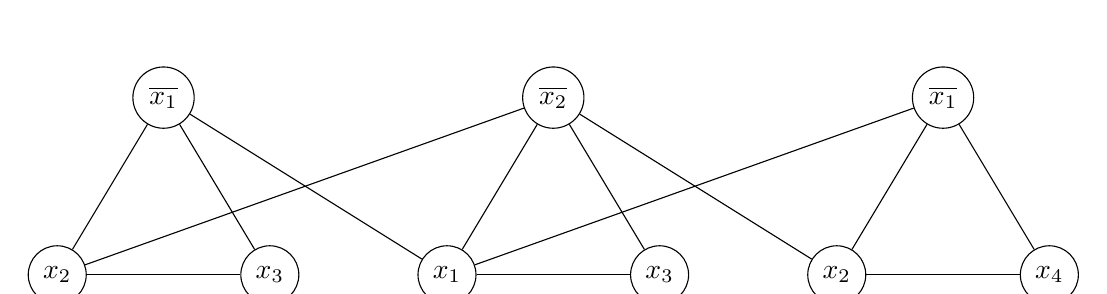
\begin{tikzpicture}  
          [scale=.9,auto=center,every node/.style={circle,draw=black}] % here, node/.style is the style pre-defined, that will be the default layout of all the nodes. You can also create different forms for different nodes.  
              
            \node (1) at (5, 2.5) {$\overline{x_1}$};  
            \node (2) at (3.5, 0) {$x_2$};  
            \node (3) at (6.5, 0) {$x_3$};

            \node (4) at (10.5, 2.5) {$\overline{x_2}$};
            \node (5) at (9, 0) {$x_1$};
            \node (6) at (12, 0) {$x_3$};

            \node (7) at (16, 2.5) {$\overline{x_1}$};
            \node (8) at (14.5, 0) {$x_2$};
            \node (9) at (17.5, 0) {$x_4$};
    
            \draw (1) -- (2);
            \draw (1) -- (3);
            \draw (2) -- (3);

            \draw (4) -- (5);
            \draw (4) -- (6);
            \draw (5) -- (6);

            \draw (7) -- (8);
            \draw (7) -- (9);
            \draw (8) -- (9);

            \draw (1) -- (5);
            \draw (5) -- (7);
            \draw (2) -- (4);
            \draw (4) -- (8);
            
        \end{tikzpicture} 
    \end{center}
    We claim that $\Phi$ is satisfiable if and only if $G$ contains 
    an independent set of size $k = |\Phi|$. 

    For the forward direction, consider any satisfying assignment for $\Phi$. 
    Then selecting one true literal from each clause (or triangle) will 
    give an independent set of size $k$. 

    Conversely, let $S$ be an independent set of size $k$. Then $S$ must 
    contain exactly one node in each triangle by construction. Set these 
    literals to ${\sf T}$ (and the remaining literals consistently). Then 
    all clauses in $\Phi$ are satisfied. This completes the proof. 
\end{pf}

The {\sc Vertex-Cover} problem is the following: given a graph $G = (V, E)$ 
and an integer $k$, is there a subset of $\leq k$ vertices such that 
each edge is incident to at least one vertex in the subset? 

The {\sc Set-Cover} problem is the following: given a set $U$ of elements, 
a collection $S$ of subsets of $U$, and an integer $k$, are there $\leq k$ 
of these subsets whose union is equal to $U$? 

\begin{theo}{theo:3.3}
    We have $\textsc{Vertex-Cover} \leq_P \textsc{Set-Cover}$. 
\end{theo}
\begin{pf}
    Given a {\sc Vertex-Cover} instance with the graph $G = (V, E)$ and 
    integer $k$, we construct a {\sc Set-Cover} instance $(U, S, k)$ that 
    has a set cover of size $k$ if and only if $G$ has a vertex cover of 
    size $k$. 

    We do this by setting the universe to be $U = E$, and include a 
    subset for each node $v \in V$ by 
    \[ S_v = \{e \in E : e \text{ incident to } v\}. \] 
    For example, consider the following graph $G$, which has a vertex 
    cover of size $2$ given by $\{c, f\}$. 
    \begin{center}
        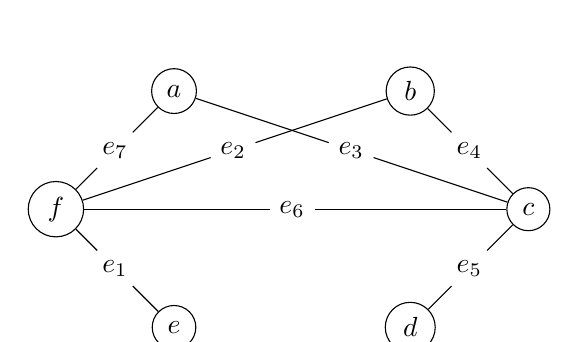
\begin{tikzpicture}              
            \node [circle, draw=black] (a) at (5, 3) {$a$};  
            \node [circle, draw=black] (b) at (8, 3) {$b$}; 
            \node [circle, draw=black] (c) at (9.5, 1.5) {$c$}; 
            \node [circle, draw=black] (d) at (8, 0) {$d$}; 
            \node [circle, draw=black] (e) at (5, 0) {$e$}; 
            \node [circle, draw=black] (f) at (3.5, 1.5) {$f$};

            \node (e1) at (4.25, 0.75) {$e_1$};
            \node (e2) at (5.75, 2.25) {$e_2$};
            \node (e3) at (7.25, 2.25) {$e_3$};
            \node (e4) at (8.75, 2.25) {$e_4$};
            \node (e5) at (8.75, 0.75) {$e_5$};
            \node (e6) at (6.5, 1.5) {$e_6$};
            \node (e7) at (4.25, 2.25) {$e_7$};

            \draw (e) -- (e1) -- (f);
            \draw (f) -- (e2) -- (b);
            \draw (a) -- (e3) -- (c);
            \draw (b) -- (e4) -- (c);
            \draw (c) -- (e5) -- (d);
            \draw (f) -- (e6) -- (c);
            \draw (f) -- (e7) -- (a);           
        \end{tikzpicture} 
    \end{center}
    Then we have universe $U = \{1, 2, 3, 4, 5, 6, 7\}$ with subsets 
    $S_a = \{3, 7\}$, $S_b = \{2, 4\}$, $S_c = \{3, 4, 5, 6\}$, 
    $S_d = \{5\}$, $S_e = \{1\}$, and $S_f = \{1, 2, 6, 7\}$. We can 
    see that $U = S_c \cup S_f$, so there is a set cover of size $2$. 

    Let us now show that $G = (V, E)$ contains a vertex cover of size $k$ 
    if and only if $U$ has a set cover of size $k$. 

    For the forward direction, let $X \subseteq V$ be a vertex cover of 
    size $k$ in $G$. Then $Y = \{S_v : v \in X\}$ is a set cover of size $k$. 
    Conversely, if $Y \subseteq S$ is a set cover of size $k$ for $U$, then 
    $X = \{v : S_v \in Y\}$ is a vertex cover of size $k$ in $G$. 
\end{pf}

\subsection{Intractability}\label{subsec:3.2}
There are three main types of problems. 
\begin{itemize}
    \item {\bf Decision problems.} Does there \emph{exist} a vertex cover of 
    size $\leq k$?
    \item {\bf Search problems.} \emph{Find} a vertex cover of size $\leq k$. 
    \item {\bf Optimization problems.} \emph{Find} a vertex cover of 
    \emph{minimum} size. 
\end{itemize}
In scheduling, we are mostly concerned with optimization problems. Notice that 
decision problems are in some sense easier than search problems, which are then 
easier than optimization problems. In particular, if the decision problem 
is intractible, then both the search and optimization problems are intractible.
Because of this, we will define {\bf P}, {\bf NP}, and {\bf EXP} using decision 
problems. A decision problem is essentially a yes or no question; we want to 
answer ``yes'' if the solution exists and ``no'' if it doesn't. 

\begin{defn}{defn:3.4}
    We denote by ${\bf P}$ the set of decision problems for which there 
    exists a polynomial time algorithm to solve it. 
\end{defn}

As we mentioned earlier, there are polynomial time algorithms for shortest 
path, primality testing, and linear programming, so these problems are all 
in {\bf P}. 

\begin{defn}{defn:3.5}
    \begin{itemize}
        \item An algorithm $C(s, t)$ is a {\bf certifier} for the problem $X$ if 
        for every string $s$, we have $s \in X$ if and only if there exists a 
        string $t$ such that $C(s, t)$ returns ``yes''. We call the string $t$ 
        the {\bf certificate} for the input $s$. 
        \item We denote by {\bf NP} the set of decision problems for which there exists 
        a polynomial time certifier. The certifier $C(s, t)$ is a 
        polynomial time algorithm, and the certificate $t$ for the input 
        $s$ is of polynomial size. 
    \end{itemize}
\end{defn}

\begin{exmp}{exmp:3.6}
    For the {\sc Sat} and {\sc 3-Sat} problems, the input is a propositional 
    formula $\Phi$ in CNF. A certificate for the input $\Phi$ is an 
    assignment of truth values to the boolean variables, and a certifier 
    checks that each clause in $\Phi$ has at least one true literal. 
    Thus, $\textsc{Sat} \in {\bf NP}$ and $\textsc{3-Sat} \in {\bf NP}$. 
\end{exmp}

Finally, we can define {\bf EXP}. 

\begin{defn}{defn:3.7}
    We denote by {\bf EXP} the set of decision problems for which there 
    exists an exponential time algorithm to solve it.
\end{defn}

\newpage
Now, we show that $\Poly \subseteq \NP \subseteq \EXP$. 

\begin{prop}{prop:3.8}
    We have $\Poly \subseteq \NP$. 
\end{prop}
\begin{pf}
    Consider a problem $X$ in $\Poly$. By definition, there exists a 
    polynomial time algorithm $A(s)$ which solves $X$ given any input $s$. 
    Then take the certificate $t = \eps$ to be the empty string, and 
    set the certifier to be $C(s, t) = A(s)$, which of course runs 
    in polynomial time. 
\end{pf}

\begin{prop}{prop:3.9}
    We have $\NP \subseteq \EXP$. 
\end{prop}
\begin{pf}
    Let $X$ be a problem in $\NP$. By definition, there exists a polynomial 
    time certifier $C(s, t)$ for $X$, whose certificate $t$ satisfies 
    $|t| \leq p(|s|)$ for some polynomial $p$ and any input string $s$. 
    To solve instance $s$, we run $C(s, t)$ on all strings $t$ with 
    $|t| \leq p(|s|)$. Return ``yes'' if and only if $C(s, t)$ returns 
    ``yes'' for any of these potential certificates. 
\end{pf}

It is a known fact that $\Poly \neq \EXP$, so we either have $\Poly \neq \NP$ 
or $\NP \neq \EXP$, or both. 

We now move on to {\bf NP}-completeness. We can think of these as the 
hardest problems in $\NP$. 

\begin{defn}{defn:3.10}
    A problem $Y \in \NP$ is called {\bf $\NP$-complete} if it has the property 
    that for every $X \in \NP$, we have $X \leq_P Y$. 
\end{defn}

The following proposition says that if we find even one problem $\NP$-complete 
problem $Y$ that is also in $\Poly$, then $\Poly = \NP$. Note that $\Poly = \NP$ 
is a famous conjecture, so we have of course not found one yet. It is commonly 
agreed upon that $\Poly \neq \NP$, but it is still an open problem.

\begin{prop}{prop:3.11}
    Suppose that $Y$ is $\NP$-complete. Then $Y \in \Poly$ if and only if 
    $\Poly = \NP$. 
\end{prop}
\begin{pf}
    For the backwards direction, notice that if $\Poly = \NP$, then 
    $Y \in \Poly$ since $Y \in \NP$. On the other hand, suppose $Y \in \Poly$. 
    Consider any problem $X \in \NP$. Since $X \leq_P Y$, we have $X \in \Poly$. 
    This implies that $\NP \subseteq \Poly$, and so $\Poly = \NP$. 
\end{pf}

The following proposition gives us a recipe for proving that a problem $Y$ 
is $\NP$-complete. 
\begin{enumerate}
    \item Show that $Y \in \NP$. 
    \item Choose an $\NP$-complete problem $X$ and prove that $X \leq_P Y$. 
\end{enumerate}

\begin{prop}{prop:3.12}
    If $X$ is $\NP$-complete, $Y \in \NP$, and $X \leq_P Y$, then 
    $Y$ is also $\NP$-complete. 
\end{prop}
\begin{pf}
    Consider any problem $W \in \NP$. Then $W \leq_P X$ by the definition 
    of $\NP$-completeness and $X \leq_P Y$ by assumption, so by transitivity, 
    we obtain $W \leq_P Y$. Since $W \in \NP$ is arbitrary, we have 
    that $Y$ is $\NP$-complete. 
\end{pf}

We now give some examples of $\NP$-complete problems. It is useful to know 
them as many scheduling problems are $\NP$-complete, and we can verify 
that they are indeed $\NP$-complete via reductions. 

\begin{theo}[Cook 1971, Levin 1973]{theo:3.13}
    The problem {\sc Sat} is $\NP$-complete. 
\end{theo}

\begin{exmp}{exmp:3.14}
    The following two problems are $\NP$-complete. 
    \begin{itemize}
        \item {\sc Partition}: Given $n$ positive integers $s_1, \dots, s_n$ 
        and $b = \frac12 \sum_{j=1}^n s_j$, does there exist a subset 
        $J \subseteq I = \{1, \dots, n\}$ such that 
        \[ b = \sum_{j\in J} s_j = \sum_{j\in I\setminus J} s_j? \] 
        \item {\sc $3$-Partition}: Given $3n$ positive integers 
        $s_1, \dots, s_{3n}$, and an integer $b$ satisfying 
        $\frac{b}{4} < s_j < \frac{b}{2}$ for all $j \in \{1, \dots, 3n\}$ 
        and $b = \frac1n \sum_{j=1}^{3n} s_j$, do there exist 
        $n$ pairwise disjoint three-element subsets $S_j \subseteq 
        \{1, \dots, 3t\}$ such that 
        \[ b = \sum_{j\in J_i} s_j \] 
        for all $j \in \{1, \dots, n\}$? 
    \end{itemize}
\end{exmp}

Next, we define what it means to be $\NP$-hard. 

\begin{defn}{defn:3.15}
    An $\NP$-hard problem is one such that every problem in $\NP$ 
    reduces to it in polynomial time. 
\end{defn}

Intuitively, $\NP$-hard problems are ``at least as hard as the hardest 
problems in $\NP$''. These problems are not necessarily in $\NP$, and they 
do not have to be decision problems. 
For instance, given an $\NP$-complete decision problem, the optimization 
problem corresponding to it is $\NP$-hard. 

There are two categories of $\NP$-hard problems.  
\begin{itemize}
    \item {\bf NP-hard in the ordinary sense.} We can reduce a known 
    $\NP$-hard problem to this problem using a polynomial time algorithm, 
    and we can find an optimal solution with an algorithm of pseudo-polynomial 
    time complexity. 
    \item {\bf NP-hard in the strong sense.} We can reduce a known 
    $\NP$-hard problem to this problem using a polynomial time algorithm, 
    even if the size of the largest parameter is polynomial in the 
    input size of the problem. 
\end{itemize}

In fact, it turns out that {\sc 3-Partition} (as defined in Example~\ref{exmp:3.14})
is $\NP$-hard in the strong sense, while {\sc Partition} is only $\NP$-hard 
in the ordinary sense. 

For our purposes, we can show that a scheduling problem is $\NP$-hard 
in the ordinary sense if {\sc Partition} (or a similar problem) can be 
reduced to this problem with a polynomial time algorithm, and there 
is an algorithm with pseudo-polynomial time complexity which solves the 
scheduling problem. 

On the other hand, we can show that a scheduling problem is $\NP$-hard 
in the strong sense if {\sc 3-Partition} (or a similar problem) can be 
reduced to this problem with a polynomial time algorithm. 

\subsection{PTAS for the Knapsack Problem}\label{subsec:3.3}
A {\bf polynomial time approximation scheme (PTAS)} is a
$(1 + \eps)$-approximation algorithm for any constant $\eps > 0$. 
While a PTAS produces arbitrarily high quality solutions, the consequence 
is that it trades off accuracy for time. Here, we will give a PTAS for the 
{\sc Knapsack} problem via rounding and scaling. 

In the {\sc Knapsack} problem, we are given $n$ objects and a knapsack. 
Each item $i$ has value $v_i > 0$ and weight $w_i > 0$. The knapsack 
has weight limit $W$. The goal is to fill the knapsack as to maximize 
the total value. 

First, we formulate the {\sc Knapsack} problem as a decision problem
and give a brief sketch that it is $\NP$-complete. 
Given a set $X$, weights $w_i \geq 0$, values $v_i \geq 0$, a weight 
limit $W$, and a target value $V$, is there a subset $S \subseteq X$ 
such that $\sum_{i\in S} w_i \leq W$ and $\sum_{i\in S} v_i \geq V$? 

The {\sc Subset-Sum} problem is the following: given $n$ natural numbers 
$w_1, \dots, w_n$ and an integer $W$, is there a subset that adds up to 
exactly $W$?

We know that {\sc Sat} is $\NP$-complete, and one can show that 
\[ \textsc{Sat} \leq_P \textsc{Subset-Sum} \leq_P \textsc{Knapsack}. \] 
\newpage
\section{More Single Machine Models} \label{sec:4}

\subsection{Maximum Lateness with Release Dates} \label{subsec:4.1}
We have already seen in Section~\ref{subsec:2.3} that there is a polynomial 
time algorithm to solve $(1\;\|\;L_{\max})$ instances. This was the 
Earliest Due Date (EDD) rule, which placed the jobs in increasing order of the 
due dates. We also saw that this was a special case of $(1 \mid \text{prec} 
\mid h_{\max})$, for which there was also an efficient algorithm, namely 
Lowest Cost Last (LCL). 

But what if we introduce release dates to the $(1\;\|\;L_{\max})$ problem? 
It turns out that this generalization, without preemption, is significantly 
harder than the problem where all jobs are available at time $0$. Moreover, 
the optimal schedule is not necessarily a non-delay schedule. It can be 
advantageous in this case to keep the machine idle before the release of a 
new job. 

\begin{theo}{theo:4.1}
    The problem $(1 \mid r_j \mid L_{\max})$ is strongly $\NP$-hard. 
\end{theo}
\begin{pf}
    This proof is based on the fact that {\sc $3$-Partition} (as described 
    in Example~\ref{exmp:3.14}) reduces to $(1 \mid r_j \mid L_{\max})$. 
    Suppose that we are given integers $a_1, \dots, a_{3t}, b$ such that 
    $\frac{b}{4} < a_j < \frac{b}{2}$ and $\sum_{j=1}^{3t} a_j = t \cdot b$. 
    We construct an instance of $(1 \mid r_j \mid L_{\max})$ with 
    $n = 4t - 1$ as follows: 
    \begin{itemize}
        \item For $j = 1, \dots, t-1$, we set $r_j = jb + (j-1)$, $p_j = 1$, 
        $d_j = jb + j$. 
        \item For $j = t, \dots, 4t-1$, we set $r_j = 0$, $p_j = a_{j-t+1}$, 
        and $d_j = tb + (t-1)$. 
    \end{itemize}
    Notice that a schedule with $L_{\max} \leq 0$ exists if and only if 
    every job $j \in \{1, \dots, t-1\}$ can be processed between 
    $r_j$ and $d_j = r_j + p_j$. This can be done if and only if the remaining 
    jobs can be partitioned over the $t$ intervals of length $b$, which can be 
    done if and only if {\sc $3$-Partition} has a solution. 
\end{pf}

The $(1 \mid r_j \mid L_{\max})$ problem is important because it often 
appears as a subproblem in heuristic procedures for flow shop and job shop 
problems. A branch and bound procedure $(1 \mid r_j \mid L_{\max})$ 
can be constructed as follows. The branching process may be based on the 
fact that schedules are developed starting from the beginning of the schedule. 
There is a single node at level $0$ which is the top of the tree. At this 
node, no job has been put into any position of the sequence yet. There are 
$n$ branches going down to $n$ nodes at level $1$. Each node at this level 
has a specific job put into the first position of the schedule. Then
at each node, there are $n-1$ jobs remaining whose position in the schedule 
has yet to be determined. Hence, there are $n-1$ arcs emanating from each 
node at level $1$ to level $2$, and there are $(n-1) \times (n-2)$ nodes at 
level $2$. We could continue in this way to enumerate all possible schedules. 

However, it is not necessary to consider every remaining job as a possible 
candidate for the next position. If the jobs $j_1, \dots, j_{k-1}$ 
are scheduled as the first $k-1$ jobs at a node at level $k-1$, then 
we only need to consider job $j_k$ if 
\[ r_{j_k} < \min_{\ell \in J} \left( \max(t, r_\ell) + p_\ell \right), \] 
where $J$ denotes the set of jobs not yet scheduled and $t$ denotes the 
time job $j_k$ is supposed to start. The reason for this condition is because 
if job $j_k$ does not satisfy this inequality, then selecting the job 
which minimizes the right-hand side instead of $j_k$ does not increase the 
value of $L_{\max}$. Therefore, the branching rule is fairly easy. 

There are several ways in which bounds for nodes can be obtained. 
One easy lower bound for a node at level $k-1$ can be established by 
scheduling the remaining jobs $J$ according to the \emph{preemptive} 
EDD rule which is known to be optimal for $(1 \mid r_j, \text{prmp} \mid 
L_{\max})$, and thus provides a lower bound for the problem at hand. 
If a preemptive EDD rule results in a non-preemptive schedule, then 
all nodes with a higher lower bound may be disregarded. 

\begin{exmp}{exmp:4.2}
    Consider the following instance of $(1 \mid r_j \mid L_{\max})$ with 
    $n = 4$ jobs. 
    \begin{align*}
        \begin{array}{c|cccc} 
            j & 1 & 2 & 3 & 4 \\ \hline 
            p_j & 4 & 2 & 6 & 5 \\ 
            r_j & 0 & 1 & 3 & 5 \\ 
            d_j & 8 & 12 & 11 & 10 
        \end{array}
    \end{align*}
    At level $1$ of the search tree, there are four nodes, namely 
    $(1, *, *, *)$, $(2, *, *, *)$, $(3, *, *, *)$, and $(4, *, *, *)$. 
    Notice that we may discard the nodes $(3, *, *, *)$ and 
    $(4, *, *, *)$ immediately. Indeed, we have $\min_{\ell\in \{1, 2, 3, 4\}} 
    (\max(t, r_\ell) + p_\ell) = 3$ with $\ell = 2$, and we see that 
    $r_3 \geq 3$ and $r_4 \geq 3$. 

    Computing a lower bound for node $(1, *, *, *)$ according to the 
    preemptive EDD rule results in a schedule where job $3$ is processed 
    during the interval $[4, 5]$, job $4$ is processed during $[5, 10]$, 
    job $3$ again during $[10, 15]$, and job $2$ during $[15, 17]$. 
    Then $L_{\max} = 5$ for this schedule, and so $5$ is a lower bound 
    for the node $(1, *, *, *)$. A similar computation shows that a lower 
    bound for the node $(2, *, *, *)$ is $7$. 

    Consider now the node $(1, 2, *, *)$ at level $2$. The lower bound 
    for this node is $6$ and is determined by the non-preemptive 
    schedule $1, 2, 4, 3$. Next, looking at the node $(1, 3, *, *)$ 
    at level $2$, the lower bound is $5$ and is determined by the 
    non-preemptive schedule $1, 3, 4, 2$. Since the lower bound for node 
    $(1, *, *, *)$ is $5$ and the lower bound for $(2, *, *, *)$ is 
    greater than $5$, it follows that the schedule $1, 3, 4, 2$ is optimal. 
\end{exmp}

The problem $(1 \mid r_j, \text{prec} \mid L_{\max})$ can be handled in a similar 
way. From an enumeration point of view, it is even easier than the problem 
without precedence constraints since many schedules can be ruled out 
immediately. 

\subsection{Number of Tardy Jobs} \label{subsec:4.2}
Recall that $U_j = 0$ if the job is timely and $U_j = 1$ if the job is late. 
The goal of the problem $(1\;\|\;\sum U_j)$ is to minimize the number of 
tardy jobs. This objective may at first appear somewhat artificial and 
seems to be of no practical interest. However, in the real world, it is a 
performance measure that is often monitored. It is equivalent to the 
percentage of on time shipments.

Notice that it does not matter how late a job is; the only 
determining factor is if it is late or not. A solution to this problem can 
be represented as a partition of the jobs into sets $S_1$ and $S_2$, where 
$S_1$ is the set of jobs meeting their due dates in Earliest Due Date (EDD)
order, and $S_2$ is the set of late jobs in an arbitrary order (since the 
amount of lateness is irrelevant).  

\begin{lemma}{lemma:4.3}
    Let OPT denote the optimal value for a given instance of $(1\;\|\;\sum U_j)$.
    If the sequence given by the EDD rule has a late job, then $\text{OPT} \geq 1$. 
\end{lemma}
\begin{pf}
    Let $k$ be the first late job in the EDD sequence. Then we have 
    \[ C_k = \sum_{i\in[k]} p_i > d_k = \max_{i\in[k]} d_i. \] 
    Consider any schedule $S$. Let $\ell$ be the last of the jobs in $[k]$ in 
    $S$. Then the completion time of $\ell$ in $S$ is at least $\sum_{i\in[k]} 
    p_i > d_\ell$, so $\ell$ is a late job in $S$. 
\end{pf}

\begin{algo}[Moore-Hodgson]{algo:4.4}
    \begin{enumerate}
        \item Enumerate the jobs in EDD order. 
        \item Set $S_1 \gets \varnothing$ and $t \gets 0$. 
        \item for $j=1$ to $n$ do: 
        \begin{itemize}[\label{}]
            \item Set $S_1 \gets S_1 \cup \{j\}$ and $t \gets t + p_j$. 
            \item if $t > d_j$ then: 
            \begin{itemize}[\label{}]
                \item Find a job $k$ with the largest $p_k$ value in $S_1$. 
                \item Set $S_1 \gets S_1 \setminus \{k\}$ and $t \gets t - p_k$. 
            \end{itemize}
            endif
        \end{itemize}
        endfor
    \end{enumerate}
\end{algo}

The principle of the Moore-Hodgson algorithm is that we schedule the jobs by the EDD 
rule, and when a job gets late, we rescue the situation by throwing out the job with 
the highest processing time. All removed jobs are considered late, and the remaining 
ones are timely. This algorithm runs in $O(n\log n)$ time. 

\begin{exmp}{exmp:4.5}
    Consider the following instance of $(1 \;\|\; \sum U_j)$ with $n = 5$ jobs, 
    where the jobs are already in EDD order.  
    \begin{align*}
        \begin{array}{c|ccccc}
            j   & 1 & 2  & 3  & 4  & 5 \\ \hline 
            p_j & 7 & 8  & 4  & 6  & 6 \\ 
            d_j & 9 & 17 & 18 & 19 & 21
        \end{array}
    \end{align*}
    We can initially schedule jobs $1$ and $2$, which will both be timely. However, 
    once we schedule job $3$, we see that it will be late, since $t = 19 > 18 = d_3$.
    \begin{verbatim}
        |---1---|---2----|-3--|
        0       7        15   19
    \end{verbatim}
    \vspace{-1em}
    Therefore, we toss out job $2$ which has the highest processing time of $p_2 = 8$
    and continue. We can schedule job $4$ just fine, but job $5$ will be late with 
    $t = 23 > 21 = d_5$. 
    \begin{verbatim}
        |---1---|-3--|--4---|--5---|
        0       7    11     17     23
    \end{verbatim}
    \vspace{-1em}
    This time, we toss out job $1$ since it has the highest processing time of $p_1 = 7$. 
    Then we obtain $S_1 = \{3, 4, 5\}$ and $S_2 = \{1, 2\}$, so $\text{OPT} = 2$ for 
    this instance. 
\end{exmp}

The following lemma is the key to proving that the Moore-Hodgson algorithm is 
optimal for $(1\;\|\;\sum U_j)$. We will assume that the jobs are already scheduled 
in EDD. 

\begin{lemma}{lemma:4.6}
    Suppose there is at least one late job in the EDD sequence $1, \dots, n$. 
    Let $k$ be the first late job in the EDD sequence, and let $m$ be the first 
    job rejected by the Moore-Hodgson algorithm. Then there is an optimal 
    schedule which rejects $m$. 
\end{lemma}
\begin{pf}
    Consider any optimal schedule $\pi$. Let $R_\pi \subseteq [n]$ denote 
    the subset of rejected (late) jobs, and let $A_\pi = [n] \setminus R_\pi$ 
    denote the set of timely jobs. By Lemma~\ref{lemma:4.3}, we may assume that 
    $\pi$ schedules the jobs of $A_\pi$ in EDD order, followed by the 
    jobs of $R_\pi$ in arbitrary order. 

    If $m \in R_\pi$, we are done. So suppose that $m \notin R_\pi$. 
    By Lemma~\ref{lemma:4.3}, there is a job $r \in [k]$ other than $m$ 
    that has been rejected. Consider the schedule $\sigma$ that sequences 
    the jobs in $A_\sigma = (A_\pi \setminus \{m\}) \cup \{r\}$ in EDD 
    order first, followed by the jobs in $[n] \setminus A_\sigma = 
    (R_\pi \setminus \{r\}) \cup \{m\}$ in arbitrary order. We will show that 
    $\sigma$ schedules all jobs in $A_\sigma$ on time. This will mean that 
    $\sigma$ is an optimal schedule since $|R_\sigma| = |R_\pi|$, 
    and by construction, $\sigma$ rejects $m$.

    First, the jobs in $A_\sigma \cap [k-1]$ are completed on time 
    since the EDD rule completes all jobs in $[k-1]$ on time. Next, 
    if $k \in A_\sigma$, then its completion time is at most 
    \[ \sum_{i\in[k] \setminus \{m\}} p_i \leq 
    \sum_{i\in[k-1]} p_i \leq d_{k-1} \leq d_k, \] 
    where the first inequality follows from the choice of $m$ by the 
    Moore-Hodgson algorithm which ensures that $p_m = 
    \max_{i\in[k]} p_i \geq p_k$. Finally, compared to the schedule $\pi$, 
    the completion times of the jobs in $A_\sigma \setminus [k] = 
    A_\pi \setminus [k]$ have been changed in the new schedule $\sigma$
    by $p_r - p_m \leq 0$, so these jobs are also on time. 
\end{pf}
 
\begin{theo}{theo:4.7}
    The Moore-Hodgson algorithm gives an optimal schedule for 
    $(1\;\|\;\sum U_j)$. 
\end{theo}
\begin{pf}
    We proceed by induction on $\text{OPT}$ over all instances of the problem. 

    If an instance has $\text{OPT} = 0$, then by Lemma~\ref{lemma:4.3}, the 
    Moore-Hodgson algorithm outputs the EDD sequence with no late jobs. 

    Suppose now that $I$ is an instance with $\text{OPT}(I) \geq 1$ late 
    jobs. Let $I'$ be obtained from $I$ by deleting the first job $m$ 
    which is rejected by the Moore-Hodgson algorithm. By Lemma~\ref{lemma:4.6}, 
    we have $\text{OPT}(I') = \text{OPT}(I) - 1$. By the induction hypothesis, 
    the algorithm finds an optimal schedule $S'$ for $I'$. The algorithm 
    for $I$ outputs the schedule $S$ such that $S$ is the same as $S'$ 
    except that job $m$ is added at the end as a rejected job. Clearly, 
    $S$ has at most $\text{OPT}(I') + 1 = \text{OPT}(I)$ rejected jobs 
    and hence is optimal. 
\end{pf}

\subsection{Total Tardiness} \label{subsec:4.3}
In practice, minimizing the number of tardy jobs $\sum U_j$ cannot be the 
only objective to measure how due dates are being met. Only minimizing 
the number of late jobs will force some jobs to have to wait for an 
unacceptably long time to complete. If we instead minimize the total 
tardiness, it is less likely that the wait for any given job will be 
unacceptably long. 

The problem $(1\;\|\;\sum T_j)$ has received an enormous amount of attention 
in literature. For many years, its computational complexity remained open; 
its $\NP$-hardness was only established recently in 1990. Since 
$(1\;\|\;\sum T_j)$ is $\NP$-hard in the ordinary sense, it allows for a 
pseudo-polynomial time algorithm based on dynamic programming. The 
algorithm is based on two preliminary results. 

\begin{lemma}{lemma:4.8}
    If $p_j \leq p_k$ and $d_j \leq d_k$, then there exists an optimal schedule 
    in which job $j$ is scheduled before job $k$. 
\end{lemma}
\begin{pf}
    We leave the proof as an exercise. This is a standard interchange 
    argument. 
\end{pf}

This type of result is useful when an algorithm has to be developed for
a problem that is $\NP$-hard. Such a result, often referred to as a 
{\bf dominance result} or {\bf elimination criterion}, often allows one to
disregard a fairly large number of sequences. Such a dominance result may also 
be thought of as a set of precedence constraints on the jobs. The more 
precedence constraints created through such dominance results, the easier the 
problem becomes.

In the following lemma, the sensitivity of an optimal sequence to the due
dates is considered. We consider two problem instances, both of which have 
$n$ jobs with processing times $p_1, \dots, p_n$. The first instance has 
due dates $d_1, \dots, d_n$. Let $k$ be a fixed job, and let $\hat C_k$ 
be the latest completion time of job $k$ among all optimal schedules. 
Then we set the due dates for the second instance to be 
\[ \hat d_j = \begin{cases}
    d_j, & \text{if } j \neq k, \\ 
    \max(d_k, \hat C_k), & \text{if } j = k.
\end{cases} \] 
In particular, we are only changing one piece of data, namely the 
due date of job $k$. 

\begin{lemma}{lemma:4.9}
    Any optimal sequence with respect to the second instance with due dates 
    $\hat d_1, \dots, \hat d_n$ is also optimal for the first instance 
    with due dates $d_1, \dots, d_n$. 
\end{lemma}
\begin{pf}
    We first introduce some notation. Let $\hat S$ be an optimal sequence 
    such that job $k$ has largest completion time $\hat C_k$ among 
    all optimal sequences. For an arbitrary sequence $S$, we let 
    $V(S)$ be the objective value according to the first instance 
    where job $k$ has due date $d_k$, and $V'(S)$ be the objective 
    value according to the second instance where job $k$ has due date 
    $\hat d_k$. 

    Let $S'$ be any optimal sequence for the second instance. Then we have 
    $V'(\hat S) \geq V'(S')$ since $S'$ is optimal for the second instance. 
    Moreover, we observe that 
    \[ V'(\hat S) = V(\hat S) - (\hat C_k - d_k), \] 
    or equivalently, $V(\hat S) - V'(\hat S) = \hat C_k - d_k$. Finally, 
    when we switch objectives, the most improvement we can get is 
    $\hat C_k - d_k$, so we deduce that 
    \begin{align*}
        V(S') &\leq V'(S') + (\hat C_k - d_k) \\ 
        &= V'(S') + V(\hat S) - V'(\hat S) \\ 
        &\leq V(\hat S).
    \end{align*}
    This means that $S'$ is also optimal for the first instance, so we are done. 
\end{pf}

Lemma~\ref{lemma:4.9} is quite a technical result, and it requires the 
knowledge of all optimal sequences for the first instance. 
For now, we will assume that the jobs are scheduled in EDD order 
so that $d_1 \leq \cdots \leq d_n$, and job $k$ is such that 
$p_k = \max(p_1, \dots, p_n)$. In particular, this is the job with 
the $k$-th smallest due date and largest processing time. It follows from 
Lemma~\ref{lemma:4.8} that there exists an optimal sequence in which 
jobs $1, \dots, k-1$ all appear in some order before job $k$. Of the remaining 
$n-k$ jobs, some may appear before job $k$ while some may appear after job $k$. 
The following lemma focuses on the placement of these remaining jobs. 

\begin{lemma}{lemma:4.10}
    There is an integer $\delta$ with $0 \leq \delta \leq n-k$ such that there 
    is an optimal sequence $S$ in which job $k$ is preceded by all jobs $j$ 
    with $j \leq k + \delta$ and followed by all jobs $j$ with $j > k + \delta$. 
\end{lemma}
\begin{pf}
    We only give a brief sketch here. In some optimal schedule, the jobs 
    $1, \dots, k-1$ are positioned before 
    job $k$ due to the dominance criterion from Lemma~\ref{lemma:4.8}. 
    From Lemma~\ref{lemma:4.9}, we can increase $d_k$ such that some other 
    jobs $k+1, \dots, k+\delta$ are positioned before job $k$ due to the 
    dominance criterion. 
\end{pf}

Lemma~\ref{lemma:4.10} tells us an optimal sequence looks like the concatenation 
of three subsets of jobs, namely 
\begin{enumerate}[(i)]
    \item jobs $1, \dots, k-1, k+1, \dots, k+\delta$ in some order, followed by 
    \item job $k$, followed by 
    \item jobs $k+\delta+1, \dots, n$ in some order. 
\end{enumerate}
The completion time of job $k$ under this schedule is 
\[ C_k(\delta) = \sum_{j\leq k+\delta} p_j. \] 
For the entire sequence to be optimal, it is clear that the first and third 
subsets must be optimally sequenced within themselves. This is the heart of 
a dynamic programming approach that determines an optimal sequence for a 
larger set of jobs after having determined optimal sequences for proper 
subsets of the larger set. 

We define $J(j, \ell, k)$ to be the set of all jobs in the set $\{j, \dots, \ell\}$ 
with processing time at most $p_k$, but $k \notin J(j, \ell, k)$. 
Note that here, $k$ does not necessarily have to be the job with highest processing 
time. Then, we define $V(J(j, \ell, k), t)$ to be the total tardiness of 
the jobs $J(j, \ell, k)$ in an optimal sequence that starts at time $t$. 
We now state the dynamic programming algorithm. 

\begin{algo}[Dynamic Programming for Total Tardiness]{algo:4.11}
    The initial conditions are $V(\varnothing, t) = 0$ and 
    $V(\{j\}, t) = \max(0, t + p_j - d_j)$ for all jobs $j$ and $t \geq 0$. 
    We have the recursive relation 
    \[ V(J(j, \ell, k), t) = \min_{\delta} \{V(J(j, k'+\delta, k'), t)
    + \max(0, C_{k'}(\delta) - d_{k'}) + V(J(k'+\delta+1, \ell, k'), 
    C_{k'}(\delta))\}, \] 
    where job $k'$ is such that $p_{k'} = \max_{j'\in J(j,\ell, k)} p_{j'}$. 
    The optimal value is then given by $V(\{1, \dots, n\}, 0)$. 
\end{algo}

Note that there are at most $O(n^3)$ subsets of jobs $J(j, \ell, k)$ and 
$\sum p_j$ possible values of $t$. This means that there are 
$O(n^3 \sum p_j)$ recursive equations. Each recursion takes $O(n)$ time, 
so the total running time of the dynamic programming approach is 
$O(n^4 \sum p_j)$, which is pseudo-polynomial. 

\begin{exmp}{exmp:4.12}
    We run our dynamic programming algorithm on an example. Consider 
    the following instance of $(1\;\|\;\sum T_j)$ with $n = 5$ jobs. 
    \begin{align*}
        \begin{array}{c|ccccc}
            j & 1 & 2 & 3 & 4 & 5 \\ \hline 
            p_j & 121 & 79 & 147 & 83 & 130 \\ 
            d_j & 260 & 266 & 266 & 336 & 337 
        \end{array}
    \end{align*}
    We see that job $3$ has the largest processing time, giving us 
    $0 \leq \delta \leq 5 - 3 = 2$. Then we have 
    \[ V(\{1, 2, 3, 4, 5\}, 0) = \min\begin{cases} 
        V(J(1, 3, 3), 0) + 81 + V(J(4, 5, 3), 347), & \text{for } \delta = 0, \\ 
        V(J(1, 4, 3), 0) + 164 + V(J(5, 5, 3), 430), & \text{for } \delta = 1, \\ 
        V(J(1, 5, 3), 0) + 294 + V(\varnothing, 560), & \text{for } \delta = 2. 
    \end{cases} \] 
    We see that $V(J(1, 3, 3), 0) = 0$ via the sequences $1, 2$ and $2, 1$. 
    The dominance rule tells us that the sequences $1, 2, 4$ and $2, 1, 4$ 
    are optimal for the jobs $J(1, 4, 3)$ with $V(J(1, 4, 3), 0) = 0$, 
    and similarly, the sequences $1, 2, 4, 5$ and $2, 1, 4, 5$ are optimal for 
    $J(1, 5, 3)$ with $V(J(1, 5, 3), 0) = 76$.

    On the other hand, we have 
    \[ V(J(4, 5, 3), 347) = (347 + 83 - 336) + (347 + 83 + 130 - 337) = 317 \] 
    for the sequence $4, 5$, and $V(J(5, 5, 3), 430) = 430 + 130 - 337 = 223$.

    Putting everything together, we obtain 
    \[ V(\{1, 2, 3, 4, 5\}, 0) = 
    \min\{0 + 81 + 317, 0 + 164 + 223, 76 + 294 + 0\}
    = \min\{398, 387, 370\} = 370. \] 
    The sequences that attain this value are $1, 2, 4, 5, 3$ and $2, 1, 4, 5, 3$.    
\end{exmp}

Since $(1\;\|\;\sum T_j)$ is $\NP$-hard, we cannot hope to find a polynomial 
time algorithm to solve arbitrary instances of it. However, we can give an FPTAS
to obtain a solution that is close to optimal, using a similar approach 
as we did for the {\sc Knapsack} problem in Section~\ref{subsec:3.4}. 

First, we will give some lower and upper bounds for total tardiness. 
\begin{itemize}
    \item Recall that the EDD rule produces a schedule with optimal 
    maximum lateness. In particular, this also produces a schedule 
    with optimal maximum tardiness. 
    \item Clearly, at least one job in a schedule has the maximum tardiness. 
    Then the total tardiness of an optimal schedule is at least the 
    optimal maximum tardiness. 
    \item The total tardiness of the EDD schedule is at least the optimal 
    maximum tardiness, but at most $n$ times the optimal maximum tardiness. 
\end{itemize}
Let $\sum T_j(\text{EDD})$ denote the total tardiness under the EDD schedule, 
and let $T_{\max}(\text{EDD}) = \max(T_1, \dots, T_n)$ be the maximum 
tardiness under the EDD schedule. For an optimal schedule $\text{OPT}$, we have 
\[ T_{\max}(\text{EDD}) \leq \sum T_j(\text{OPT}) \leq \sum T_j(\text{EDD}) 
\leq n \cdot T_{\max}(\text{EDD}). \] 
Let $V(J, t)$ be the minimum total tardiness of the job subset $J$ 
assuming that processing begins at time $t$. There is a time $t^*$ 
such that $V(J, t) = 0$ for all $t \leq t^*$ and $V(J, t) > 0$ for all 
$t > t^*$. Then we have $V(J, t^* + \delta) \geq \delta$ for all 
$\delta \geq 0$. By executing the pseudo-polynomial dynamic programming 
approach described in Algorithm~\ref{algo:4.11}, one only has to compute 
$V(J, t)$ for 
\[ \max\{0, t^*\} \leq t \leq t^* + n \cdot T_{\max}(\text{EDD}). \] 
Substituting $\sum p_j$ in the overall running time of the dynamic 
programming algorithm by $n \cdot T_{\max}(\text{EDD})$ yields a 
new bound of $O(n^5 \cdot T_{\max}(\text{EDD}))$. 

Now, rescale the processing times and due dates via $p'_j = 
\lfloor p_j/K \rfloor$ and $d'_j = d_j/K$ for some factor $K > 0$. 
Let $S$ be an optimal schedule for the rescaled problem. We let 
$\sum T_j^*(S)$ denote the total tardiness of the schedule $S$ with 
respect to the processing times $Kp'_j \leq p_j$ and due dates $d_j$. 
Let $\sum T_j(S)$ denote the total tardiness of the schedule $S$ with 
respect to the original processing times $p_j$ and due dates $d_j$. 
From the fact that $Kp'_j \leq p_j < K(p'_j + 1)$, it follows that 
\[ \sum T_j^*(S) \leq \sum T_j(\text{OPT}) \leq \sum T_j(S) < 
\sum T_j^*(S) + \frac{Kn(n+1)}{2}. \] 
This chain of inequalities implies that 
\[ \sum T_j(S) - \sum T_j(\text{OPT}) < \frac{Kn(n+1)}{2}. \] 
If $K$ is chosen such that 
\[ K = \frac{2\eps}{n(n+1)} \cdot T_{\max}(\text{EDD}), \] 
then we obtain 
\[ \sum T_j(S) - \sum T_j(\text{OPT}) < \eps \cdot T_{\max}(\text{EDD}). \] 
Moreover, for this choice of $K$, the time bound 
$O(n^5 \cdot T_{\max}(\text{EDD})/K)$ becomes $O(n^7/\eps)$, making 
our approximation scheme fully polynomial. We summarize the FPTAS 
as follows. 

\begin{algo}[Total Tardiness FPTAS]{algo:4.13}
    \begin{enumerate}[(1)]
        \item Apply EDD in order to determine $T_{\max}(\text{EDD})$. 
        If $T_{\max}(\text{EDD}) = 0$, then $\sum T_j(\text{OPT}) = 0$ 
        and EDD gives an optimal schedule, so stop. Otherwise, set 
        \[ K = \frac{2\eps}{n(n+1)} \cdot T_{\max}(\text{EDD}). \] 
        \item Rescale the processing times and due dates via 
        $p'_j = \lfloor p_j/K \rfloor$ and $d'_j = d_j/K$. 
        \item Apply Algorithm~\ref{algo:4.11} to the rescaled data. 
    \end{enumerate}
\end{algo}

\subsection{Weighted Number of Late Jobs} \label{subsec:4.4}
The generalization of the problem $(1\;\|\;\sum U_j)$ with additional weights 
is known to be $\NP$-hard. This can be shown via a reduction from 
{\sc $3$-Partition}. A popular heuristic for this problem is the WSPT rule, 
but even that can perform very badly. As usual, we cannot hope to find a 
polynomial time algorithm which solves $(1\;\|\;\sum w_j U_j)$. 

\begin{exmp}{exmp:4.14}
    Consider the following instance of $(1 \mid d_j = d \mid \sum w_j U_j)$ with 
    $n = 3$ jobs and equal due dates. 
    \begin{align*}
        \begin{array}{c|ccc}
            j & 1 & 2 & 3 \\ \hline 
            p_j & 11 & 9 & 90 \\ 
            d_j & 100 & 100 & 100 \\ 
            w_j & 12 & 9 & 89
        \end{array}
    \end{align*}
    Then the WSPT rule fails: it gives the schedule $1, 2, 3$ which has 
    objective value $89$. The optimal schedules for this example are 
    $2, 3, 1$ and $3, 2, 1$, which both have objective value $12$. 
\end{exmp}

In fact, the {\sc Knapsack} problem is equivalent to the special case 
$(1 \mid d_j = d \mid \sum w_j U_j)$ where all due dates are equal. 
Indeed, we can think of the due date $d$ as the weight of the knapsack, 
the processing times $p_j$ as the weight of the individual items, 
and the weights $w_j$ as their values. We then want to minimize the value 
of the items we are throwing out of the knapsack, which is the same 
as maximizing the value of the items inside the knapsack. 

In this section, our goal is to come up with some dynamic programming 
approaches to solve $(1\;\|\;\sum w_j U_j)$ in pseudo-polynomial time. 
We then construct an FPTAS using one of the dynamic programming schemes. 

First, we will introduce some notation. Consider an instance of 
$(1\;\|\;\sum w_j U_j)$ where all weights $w_j \geq 0$ are integer. 
We assume that the jobs are indexed by the EDD sequence. 
\begin{itemize}
    \item We call $S$ a {\bf feasible} set of jobs if every job in $S$ 
    can be completed on time starting at time $0$. 
    \item We define $w(S) = \sum_{j\in S} w_j$ and $p(S) = \sum_{j\in S} p_j$. 
\end{itemize}

{\bf Approach 1.} We define $T(i, \hat w)$ to be the minimum completion 
time of a feasible subset $S$ of $[i] = \{1, \dots, i\}$ with weight 
$\geq \hat w$. We can think of $\hat w$ as a ``target'' weight. 
In other words, $T(i, \hat w)$ is the minimum completion time of a 
chosen subset of the jobs $\{1, \dots, i\}$ such that all jobs in the 
chosen subset are timely (that is, there are no late jobs in an EDD ordering 
of the chosen subset) and moreover, the total weight of the jobs in the 
chosen subset is $\geq \hat w$.

We set $T(i, \hat w) = \infty$ if no such feasible set exists, 
$T(0, 0) = 0$, and $T(0, \hat w) = \infty$ for all $\hat w > 0$. Then 
the recurrence relation is given by 
\[ T(i, \hat w) = \begin{cases}
    \min\{T(i-1, \hat w), p_i + T(i-1, \hat w - w_i)\}, & \text{if } 
    p_i + T(i-1, \hat w - w_i) \leq d_i, \\ 
    T(i-1, \hat w), & \text{otherwise.} 
\end{cases} \] 
In the computed table for $T(i, \hat w)$, there are $n+1$ rows corresponding 
to $i = 0, \dots, n$ where $n$ is the number of jobs, and $\sum w_j + 1$ 
corresponding to the potential total weights $\hat w = 0, \dots, \sum w_j$. 
From the table, we can then find the optimal solution to the 
$(1\;\|\;\sum w_j U_j)$ instance in $O(\sum w_j)$ time.

We can actually do slightly better. If $w^*$ is the maximum value of 
$w$ such that $T(i, w^*)$ is finite, then we can compute the table for 
$T(i, \hat w)$ in $O(nw^*)$ time and find the optimal solution from the 
table in $O(w^*)$ time. So the dynamic programming algorithm runs in time 
$O(nw^*)$. 

{\bf Approach 2.} This is the approach we will use for our FPTAS. We define 
$Q(i, \hat w)$ to be the minimum completion time of a feasible subset $S$ 
of $[i]$ such that $w([i] \setminus S) \leq \hat w$. In other words, 
$Q(i, \hat w)$ is the minimum completion time of a chosen subset of the jobs 
$\{1, \dots, i\}$ such that all of the jobs in the chosen subset are timely 
(that is, there are no late jobs in an EDD ordering of the chosen subset)
and moreover, the sum of the weights of the remaining jobs in 
$\{1, \dots, i\}$ is $\leq \hat w$. 

We define $Q(0, \hat w) = 0$ for all $\hat w \geq 0$ and $Q(0, \hat w) 
= \infty$ for all $\hat w < 0$. Then the recurrence relation is given by 
\[ Q(i, \hat w) = \begin{cases}
    \min\{Q(i-1, \hat w - w_i), p_i + Q(i-1, \hat w)\}, & \text{if } 
    p_i + Q(i-1, \hat w) \leq d_i, \\ 
    Q(i-1, \hat w - w_i), & \text{otherwise.}
\end{cases} \]
In essence, this is the complement to the first approach. But why do we 
prefer this one instead? This is because it is slightly more efficient. 
We do not need to compute all of the entries of the table like in the 
first approach; we only need to start at $\hat w = 0$ and stop when 
we reach the minimum value $w^{**}$ such that $Q(i, w^{**})$ is finite. 
Observe that this minimum value $w^{**}$ is the same as the optimal value 
to the $(1\;\|\;\sum w_j U_j)$ instance. In many cases, the value of 
$w^{**}$ is much smaller than that of $w^*$ above. 

Our FPTAS then uses an extension of the above observation. If we can compute a 
lower bound $\text{LB}$ on $\text{OPT}$ such that $\text{LB} \leq 
\text{OPT} \leq n \cdot \text{LB}$, then we could replace $w^{**}$ above 
by $n \cdot \text{LB}$. We design the FPTAS by scaling and rounding the 
weights, and then applying our second dynamic programming approach above
with $Q(i, \hat w)$. This is quite similar to the FPTAS of the {\sc Knapsack} 
problem. 

There are two key building blocks for the FPTAS for $(1\;\|\;\sum w_j U_j)$. 
\begin{enumerate}[(1)]
    \item We need a lower bound $\text{LB}$ on $\text{OPT}$ computable in 
    polynomial time such that $\text{LB} \leq \text{OPT} \leq n \cdot \text{LB}$.
    \item We need an algorithm (based on dynamic programming) which computes 
    the optimal value and runs in time  polynomial in $n$ and $\text{LB}$. 
\end{enumerate}
We address (1) by solving the problem $(1\;\|\;\max_j w_jU_j)$ on the 
same instance. This can be done by applying the LCL algorithm 
(Algorithm~\ref{algo:2.10}) to the functions 
\[ h_j(C_j) = \begin{cases} 
    0, & \text{if } C_j \leq d_j, \\ 
    w_j, & \text{if } C_j > d_j. 
\end{cases} \] 
We also have the following result, and we leave its proof as an exercise. 

\begin{prop}{prop:4.15}
    For any schedule $S$, we have 
    \[ \max_j w_j U_j^S \leq \sum_j w_j U_j^S \leq n \cdot \max_j w_j U_j^S. \] 
    Moreover, if $S^*$ is an optimal schedule for $(1\;\|\;\max_j w_jU_j)$, then 
    \[ \max_j w_j U_j^{S^*} \leq \text{OPT} \leq n \cdot \max_j w_j U_j^{S^*}, \] 
    where $\text{OPT}$ is the optimal value for the $(1\;\|\;\sum w_j U_j)$ instance. 
\end{prop}

We set $\text{LB}$ to be the optimal value for the $(1\;\|\;\max_j w_j U_j)$ 
instance. Our scale and round step is straightforward. Given an error 
parameter $\eps > 0$, let the scaling parameter be $\delta = \eps \cdot 
\text{LB}/n$. We define $w'_j = \lfloor w_j/\delta \rfloor$ for all jobs $j$. 
It is easy to see that $w_j/\delta - 1 \leq w'_j \leq w_j/\delta$. 

We apply the second dynamic programming algorithm to the rounded instance 
with the weights $w'$. The running time is polynomial in $n$ and 
$\text{LB}'$ where $\text{LB}' = \text{LB}/\delta = n/\eps$ because 
the optimal value of the rounded instance is $\leq n \cdot \text{LB}'$.

For the rounded instance, let $\text{OPT}'$ denote the optimal value. 
Let $A'$ be the set of late jobs in an optimal schedule, so $w'(A') = 
\text{OPT}'$. Let $A^*$ be the set of late jobs in an optimal schedule for 
the original instance so that $w(A^*) = \text{OPT}$. 

We claim that $w(A') \leq (1+\eps) \text{OPT}$. This follows from applying some
inequalities we have stated earlier and the fact that $w'(A') \leq w'(A^*)$ 
since $A'$ is optimal for the weights $w'$. Indeed, we have 
\begin{align*} 
    w(A') &= \sum_{j\in A'} w_j \leq \sum_{j\in A'} (\delta w'_j + \delta) \\
    &\leq \delta w'(A') + n\delta \\ 
    &\leq \delta w'(A^*) + n\delta \\
    &\leq w(A^*) + \eps \cdot \text{LB} \\ 
    &\leq (1 + \eps) w(A^*) \\ 
    &= (1 + \eps) \text{OPT}. 
\end{align*}
Thus, we see that our algorithm is an FPTAS. 
\newpage
\section{Advanced Single Machine Models} \label{sec:5}

\subsection{Total Earliness and Tardiness} \label{subsec:5.1}
One could imagine a situation where an earliness penalty is incurred. For 
example, if one needs to go to convocation in a different city a week from now, 
they wouldn't want to go immediately as they would need to pay for rent 
or parking.  We define the earliness of a job $j$ by $E_j = \max(0, d_j - C_j)$.
Note that unlike the performance measures we have discussed so far, 
earliness is non-regular because it is decreasing with respect to 
completion time. 

In this section, we cover a generalization of the total tardiness 
problem. We will focus on the objective 
\[ \sum_{j=1}^n E_j + \sum_{j=1}^n T_j. \] 
Intuitively, this problem is harder than total tardiness, which is known to be 
$\NP$-hard. Therefore, we will focus on the special case where all 
jobs have the same due date $d_j = d$. 

An optimal schedule for this special case has some useful properties. For 
example, it is easily shown that there is no idleness between any two jobs 
for an optimal schedule, as one could close the gap by shifting jobs 
later if they are early, or shifting jobs earlier if they are late. 
Moreover, it is possible that an optimal schedule does not start processing 
the jobs immediately at time $0$. Indeed, by the previous property, 
an increase of $d$ would increase the starting time of the first job if 
$d$ is sufficiently large. 

We also observe that we can divide any sequence of jobs into 
two disjoint sets and possibly one additional job. One set consists of the jobs 
that are completed early so that $C_j \leq d$, and we will denote it by $J_1$. 
The other set consists of the jobs that are started late, and we will denote it 
by $J_2$. There may be another job which is started early but 
completed late. 

\begin{prop}{prop:5.1}
    There is an optimal sequence in which one job is completed exactly 
    at time $d$. 
\end{prop}
\begin{pf}
    We proceed by contradiction. Suppose there is no such schedule. Then
    there is always one job that starts its processing before time $d$ and 
    completes its processing after time $d$. Call this job $j^*$. 
    Let $|J_1|$ denote the number of jobs that are early and $|J_2|$ 
    denote the number of jobs that are late. If $|J_1| < |J_2|$, then we 
    can shift the entire schedule to the left in such a way that job $j^*$
    completes its processing exactly at time $d$. This implies that the 
    total tardiness decreases by $|J_2|$ times the length of the shift, 
    while the total earliness increases by $|J_1|$ times the length of 
    the shift. Clearly, the objective value is reduced. The case 
    where $|J_1| > |J_2|$ can be treated in a similar way. 

    The case where $|J_1| = |J_2|$ is somewhat special. In this case, there 
    are many optimal schedules, of which only two satisfy the property 
    given in the lemma. 
\end{pf}

Due to Proposition~\ref{prop:5.1}, we can avoid the situation where we have the 
additional job in the middle altogether. In particular, there is an optimal 
schedule such that the first job starts at time $0$ or later, the jobs in $J_1$ 
scheduled first according to Longest Processing Time (LPT), and the jobs in $J_2$
are scheduled last according to Shortest Processing Time (SPT). In this 
sense, the schedule is shaped like a ``V''. Note that for a schedule of the 
above form, say $1, \dots, n$, the total earliness is 
\[ \sum_{j\in J_1} E_j = 0 \cdot p_1 + 1 \cdot p_2 + 2 \cdot 
p_3 + \cdots + (|J_1| - 1) \cdot p_{|J_1|}, \] 
while the total tardiness is 
\[ \sum_{j\in J_2} T_j = 1 \cdot p_{|J_1|+|J_2|} + 2 \cdot 
p_{|J_1|+|J_2|-1} + \cdots + |J_2| \cdot p_{|J_1|+1}. \] 
For an instance in which all optimal schedules start processing the first job
some time after $t = 0$ (that is, the due date $d$ is sufficiently large), 
the following algorithm yields the optimal allocations of jobs to sets 
$J_1$ and $J_2$. We assume that the jobs are ordered such that $p_1 \geq 
p_2 \geq \cdots \geq p_n$. 

\begin{algo}[Minimizing Total Earliness and Tardiness with Loose Due Date]{algo:5.2}
    {\sc Step 1.} Assign job $1$ to set $J_1$. Initialize $k = 2$. 

    {\sc Step 2.} Assign job $k$ to set $J_1$ and job $k+1$ to set $J_2$, 
    or vice versa. 

    {\sc Step 3.} If $k+2 \leq n-1$, then increase $k$ by $2$ and go back to 
    Step 2. If $k+2 = n$, assign job $n$ to either set $J_1$ or set $J_2$ 
    and stop. If $k+2 = n+1$, then all jobs have been assigned, so we stop. 
\end{algo}

This algorithm is somewhat flexible in its assignment of jobs to sets $J_1$ and 
$J_2$. It can be implemented in a way that in the optimal assignment, the 
total processing time of the jobs assigned to $J_1$ is minimized. Given the 
total processing time of the jobs in $J_1$ and the due date $d$, it can be 
verified easily whether the machine indeed must remain idle before it starts 
processing its first job.

If the due date $d$ is tight and it is necessary to start processing 
a job at time $0$, then the problem is $\NP$-hard. The following heuristic 
which assigns the $n$ jobs to the $n$ positions in the sequence can be 
very effective, but does not always yield an optimal sequence. Again, we 
assume that $p_1 \geq p_2 \geq \cdots \geq p_n$.  

\begin{algo}[Minimizing Total Earliness and Tardiness with Tight Due Date]{algo:5.3}
    {\sc Step 1.} Initialize $\tau_1 = d$ and $\tau_2 = \sum_{j=1}^n p_j - d$. 
    Set $k = 1$.  

    {\sc Step 2.} If $\tau_1 > \tau_2$, then assign job $k$ to the first 
    unfilled position in the sequence and decrease $\tau_1$ by $p_k$. 
    If $\tau_1 < \tau_2$, then assign job $k$ to the last unfilled position 
    in the sequence and decrease $\tau_2$ by $p_k$. 

    {\sc Step 3.} If $k < n$, then increase $k$ by $1$ and go back to Step 2. 
    If $k = n$, then stop. 
\end{algo}

We give an example of this heuristic in action. 

\begin{exmp}{exmp:5.4}
    Consider the following example with $6$ jobs and common due date $d = 180$. 
    \begin{align*}
        \begin{array}{c|cccccc}
            j & 1 & 2 & 3 & 4 & 5 & 6 \\ \hline 
            p_j & 106 & 100 & 96 & 22 & 20 & 2
        \end{array}
    \end{align*}
    Applying the heuristic yields the following results. 
    \begin{align*}
        \begin{array}{c|c|c|c}
            \tau_1 & \tau_2 & \text{Assignment} & \text{Sequence} \\ \hline 
            180 & 166 & \text{Job $1$ placed first} & 1, *, *, *, *, * \\ 
            74 & 166 & \text{Job $2$ placed last} & 1, *, *, *, *, 2 \\ 
            74 & 66 & \text{Job $3$ placed first} & 1, 3, *, *, *, 2 \\ 
            -22 & 66 & \text{Job $4$ placed last} & 1, 3, *, *, 4, 2 \\ 
            -22 & 44 & \text{Job $5$ placed last} & 1, 3, *, 5, 4, 2 \\
            -22 & 24 & \text{Job $6$ placed last} & 1, 3, 6, 5, 4, 2 \\  
        \end{array}
    \end{align*}
\end{exmp}

To end this section, we discuss some other versions of total 
earliness and tardiness problems. 
\begin{itemize}

    \item Consider the objective $\sum w'E_j + \sum w''T_j$ where all 
    due dates are equal with $d_j = d$. All jobs have exactly the same 
    cost function, but the earliness penalty $w'$ and the tardiness 
    penalty $w''$ are not the same. All the previous properties and
    algorithms can be generalized relatively easily to take the 
    difference between $w'$ and $w''$ into account. 

    \item Consider the more general objective $\sum w'_j E_j + \sum w''_j T_j$ 
    with $d_j = d$ for all jobs $j$. In this case, the shapes of the cost 
    functions of the jobs are different. The LPT-SPT sequence described above 
    is not necessarily optimal. The first part of the sequence must now be 
    ordered according to Weighted Longest Processing Time first (WLPT), 
    which is in increasing order of $w_j/p_j$. The second part of the 
    sequence is ordered by Weighted Shortest Processing Time first (WSPT), 
    which we are already familiar with. 

    \item Consider the model with the objective function $\sum w'E_j + \sum w''T_j$
    where we do not assume that the due dates are equal. It is clear that this 
    case is $\NP$-hard as it is a more general model of the one we discussed in
    Section~\ref{subsec:4.3}. This problem has an additional level of complexity. Because of
    the different due dates, it may not necessarily be optimal to process the 
    jobs one after another without interruption; it may be necessary to have 
    idle times between the processing of consecutive jobs. Therefore, this 
    problem has two aspects: one concerning the sequencing of the jobs, 
    and the other concerning the idle time between the jobs. Approaches 
    for this problem are typically based either on dynamic programming 
    or branch and bound. However, given a predetermined sequence, the timing of 
    the processing of the jobs (and therefore also the idle times) can be 
    determined in polynomial time. This can also be applicable in a more 
    general setting, which we will describe next. 

    \item The most general setting has objective $\sum w'_j E_j + 
    \sum w''_j T_j$ where the jobs have different due dates and weights. 
    This problem is strongly $\NP$-hard since it is harder than 
    $(1~||~\sum w_j T_j)$, which is also known to be strongly $\NP$-hard.
    But again, given a predetermined sequence of the jobs, the timing 
    of the jobs can be determined in polynomial time. However, we will not 
    go into detail about this. 

\end{itemize} 

\subsection{Primary and Secondary Objectives} \label{subsec:5.2}
In practice, a scheduler is often concerned with more than one objective. 
For example, one might want to minimize inventory costs and meet due dates. 
It would then be of interest, for instance, to find a schedule that minimizes a 
combination of $\sum C_j$ and $L_{\max}$. 

In many cases, there is more than one optimal schedule that minimizes a 
given objective. A scheduler may then wish to consider the set of all 
schedules that are optimal with respect to one objective (which 
we will call the primary objective), and then search within this set of 
schedules for the schedule that is best with regard to a secondary objective. 
If the primary objective is $\gamma_1$ and the secondary objective is 
$\gamma_2$, then such a problem is denoted by 
$(\alpha~|~\beta~|~\gamma_1^{(1)}, \gamma_2^{(2)})$.

We begin with the simple example $(1~||~\sum C_j^{(1)}, L_{\max}^{(2)})$ 
where the primary objective is the total completion time and the secondary 
objective is the maximum lateness. If there are no jobs with identical 
processing times, then there is exactly one schedule that minimizes the 
total completion time (namely the one obtained by SPT), so there is 
no freedom to minimize $L_{\max}$. If there are jobs with identical processing 
times, then there are multiple schedules that minimize the total completion 
time. A set of jobs with identical processing times is preceded by a job with a 
strictly shorter processing time and followed by a job with a strictly longer
processing time. Jobs with identical processing times have to be processed 
one after another, but the key is that they may be done in any order. 
Then to minimize $L_{\max}$, we can put these jobs with identical processing 
times in EDD order. We can refer to this rule as SPT/EDD, since the jobs are 
first scheduled according to SPT and ties are broken according to EDD. This 
rule can generalized to the case where the primary objective is 
the total weighted completion time $\sum w_j C_j$. 

Consider now the problem $(1~||~\sum L_{\max}^{(1)}, C_j^{(2)})$, which 
has the same two objectives with reversed priorities. We know that 
the EDD rule minimizes $L_{\max}$; suppose that the value of this minimum 
$L_{\max}$ is $z$. Then the original problem can be transformed to 
another equivalent problem. By creating a new set of due dates 
$\overline{d_j} = d_j + z$, we see that these due dates are now deadlines. 
The problem is to find a schedule which minimizes $\sum C_j$ subject to 
the constraint that every job is completed by its deadline. We denote 
this problem by $(1~|~\text{hard } d_j~|~\sum C_j)$. The algorithm 
for finding the optimal schedule is based on the following result. 

\begin{lemma}{lemma:5.5}
    There exists a schedule that minimizes $\sum C_j$ in which job $k$ 
    is scheduled last if and only if 
    \begin{enumerate}[(1)]
        \item $\overline{d_k} \geq \sum_{j=1}^n p_j$, and 
        \item $p_k \geq p_\ell$ for all jobs $\ell$ such that 
        $\overline{d_\ell} \geq \sum_{j=1}^n p_j$. 
    \end{enumerate}
\end{lemma}
\begin{pf} 
    Assume towards a contradiction that job $k$ is not scheduled last. 
    There is a set of jobs that is scheduled after job $k$, and 
    some job $\ell$ that is scheduled last. Note that job $\ell$ 
    must satisfy condition (1) for otherwise it would not meet its due date. 
    This means that job $\ell$ does not satisfy condition (2) and 
    so $p_\ell < p_k$. After swapping jobs $k$ and $\ell$, the sum of the 
    completion times of jobs $k$ and $\ell$ decreases, and the sum of the 
    completion times of jobs scheduled between $k$ and $\ell$ also decreases. 
    Hence, the original schedule that positioned job $\ell$ last could not have 
    minimized $\sum C_j$. 
\end{pf}

In the following algorithm, $J^c$ represents the set of jobs that have 
not been scheduled yet. 

\begin{algo}[Minimizing Total Completion Time with Deadlines]{algo:5.6}
    {\sc Step 1.} Set $k = n$, $\tau = \sum_{j=1}^n p_j$, and $J^c = \{1, \dots, n\}$. 

    {\sc Step 2.} Find a job $k^* \in J^c$ such that $\overline{d_{k^*}} \geq \tau$ 
    and $p_{k^*} \geq p_\ell$ for all jobs $\ell \in J^c$ such that 
    $\overline{d_\ell} \geq \tau$. Put job $k^*$ in position $k$ of the sequence. 

    {\sc Step 3.} Decrease $k$ by $1$, decrease $\tau$ by $p_{k^*}$, and 
    delete job $k^*$ from $J^c$. 

    {\sc Step 4.} If $k \geq 1$, then go back to Step 2. Otherwise, stop. 
\end{algo}

We give a simple example of the use of this backward algorithm. 

\begin{exmp}{exmp:5.7}
    Consider the following instance of $5$ jobs. 
    \begin{align*}
        \begin{array}{c|ccccc}
            j & 1 & 2 & 3 & 4 & 5 \\ \hline 
            p_j & 4 & 6 & 2 & 4 & 2 \\ 
            d_j & 10 & 12 & 14 & 18 & 18
        \end{array}
    \end{align*}
    For ease of notation, we will let $\hat J(\tau) = \{\ell \in J^c : 
    \overline{d_\ell} \geq \tau\}$ be the set of eligible jobs that have 
    not been scheduled yet. We start with $\tau = \sum_{j=1}^5 p_j = 18$, 
    and applying the algorithm yields the following results. 
    \begin{align*}
        \begin{array}{c|c|c|c} 
            \text{Iteration} & \tau & \hat J(\tau) & k^* \\ \hline 
            1 & 18 & \{4, 5\} & 4 \\ 
            2 & 14 & \{3, 5\} & 3 \text{ or } 5 \\ 
            3 & 12 & \{2, 5\} \text{ or } \{2, 3\} & 2 \\ 
            4 & 6 & \{1, 5\} \text{ or } \{1, 3\} & 1 \\ 
            5 & 2 & \{5\} \text{ or } \{3\} & 5 \text{ or } 3            
        \end{array}
    \end{align*}
    Thus, we obtain two optimal schedules, which are $5, 1, 2, 3, 4$ and 
    $3, 1, 2, 5, 4$. 
\end{exmp}

It can be shown that even when preemptions are allowed, the optimal schedules 
are non-preemptive for the $(1~|~\text{hard } d_j~|~\sum C_j)$ problem. We can 
also assume feasibility of the problem in general as it can be checked easily 
using the EDD rule. 

Finally, we note that a fairly large number of problems of the form 
$(1~|~\beta~|~\gamma_1^{(1)}, \gamma_2^{(2)})$ have been studied in the 
literature. Very few of them can be solved in polynomial time. However, 
problems of the type $(1~|~\beta~|~\sum w_j C_j^{(1)}, \gamma_2^{(2)})$ 
tend to be easy based on the analysis of the $(1~||~\sum C_j^{(1)}, 
L_{\max}^{(2)})$ problem we discussed at the beginning of the lecture. 
We will see one such example on Assignment 6.

\subsection{Parametric Analysis of Multiple Objectives} \label{subsec:5.3}
Suppose that we have the two objectives $\gamma_1$ and $\gamma_2$. If 
the overall objective is $\theta_1 \gamma_1 + \theta_2 \gamma_2$ where 
$\theta_1$ and $\theta_2$ are the weights of the two objectives, then 
we can denote the scheduling problem by $(1~|~\beta~|~\theta_1 \gamma_1 
+ \theta_2 \gamma_2)$. Multiplying both weights by the same constant 
does not change the problem, so we may assume without loss of generality 
that $\theta_1 + \theta_2 = 1$. For this section, we will focus on a 
specific class of schedules. 

\begin{defn}{defn:5.8}
    A schedule is called {\bf Pareto optimal} if it is not possible to 
    decrease the value of one objective without increasing the value of 
    the other. 
\end{defn}

All Pareto optimal schedules can be represented by a set of points in the 
$(\gamma_1, \gamma_2)$ plane. This set of points illustrates the tradeoffs 
between the two objectives. Consider the two objectives we analyzed in the 
previous section, namely $\sum C_j$ and $L_{\max}$. The two cases 
we covered are the two extreme points of the tradeoff curve. Note that 
if $\theta_1 \to 0$ and $\theta_2 \to 1$, then 
\[ (1~|~\beta~|~\theta_1\gamma_1 + \theta_2\gamma_2) \to 
(1~|~\beta~|~\gamma_2^{(1)}, \gamma_1^{(2)}), \] 
while if $\theta_2 \to 0$ and $\theta_1 \to 1$, then 
\[ (1~|~\beta~|~\theta_1\gamma_1 + \theta_2\gamma_2) \to 
(1~|~\beta~|~\gamma_1^{(1)}, \gamma_2^{(2)}). \] 
We will now focus on generating all Pareto optimal schedules for the 
problem $(1~||~\theta_1 \sum C_j + \theta_2 L_{\max})$. 

On one end of the extremes is the $(1~||~\sum L_{\max}^{(1)}, \sum C_j^{(2)})$ 
problem, which could be solved using a more complicated backward algorithm
where we have $L_{\max} = L_{\max}(\text{EDD})$. 

On the other end, we have the $(1~||~\sum C_j^{(1)}, L_{\max}^{(2)})$ problem, 
where the total completion time was minimized by the SPT rule and ties were 
broken by EDD. We denoted this strategy by SPT/EDD, and we easily see that 
$L_{\max} = L_{\max}(\text{SPT/EDD})$ in this case. It is clear that 
\[ L_{\max}(\text{EDD}) \leq L_{\max}(\text{SPT/EDD}). \] 
The algorithm that generates all Pareto optimal solutions in the tradeoff 
curve contains two loops. One series of steps in the algorithm (the inner 
loop) is an adaptation of Algorithm~\ref{algo:5.6}. In addition to the optimal 
schedule with a maximum allowable $L_{\max}$, these steps determine 
the minimum increment $\delta$ in the $L_{\max}$ that would allow for a 
decrease in the minimum $\sum C_j$. The second (outer) loop of the algorithm 
contains the structure that generates all the Pareto optimal points.
The outer loop calls the inner loop at each Pareto optimal point to generate a 
schedule at that point and also to determine how to move to the next efficient 
point. The algorithm starts out with the EDD schedule that generates the first
Pareto optimal point in the upper left part of the trade-off curve. It 
determines the minimum increment in the $L_{\max}$ needed to achieve a 
reduction in $\sum C_j$. Given this new value of $L_{\max}$, it uses 
Algorithm~\ref{algo:5.6} to determine the schedule which minimizes 
$\sum C_j$, and proceeds to determine the next increment. This goes on 
until the algorithm reaches $L_{\max}(\text{SPT/EDD})$. 

\begin{algo}[Tradeoffs between Total Completion Time and 
    Maximum Lateness]{algo:5.9}
    {\sc Step 1.} Set $r = 1$. Set $L_{\max} = L_{\max}(\text{EDD})$ and 
    $\overline{d_j} = d_j + L_{\max}$. 

    {\sc Step 2.} Set $k = n$ and $J^c = \{1, \dots, n\}$. Set 
    $\tau = \sum_{j=1}^n p_j$ and $\delta = \tau$. 

    {\sc Step 3.} Find a job $j^* \in J^c$ such that $\overline{d_{j^*}} \geq \tau$ 
    and $p_{j^*} \geq p_\ell$ for all jobs $\ell \in J^c$ such that 
    $\overline{d_\ell} \geq \tau$. Put job $j^*$ in position $k$ of the 
    sequence. 

    {\sc Step 4.} If there is no job $\ell$ such that $\overline{d_\ell} < 
    \tau$ and $p_\ell > p_{j^*}$, then go to Step 5. Otherwise, let 
    \[ \delta^{**} = \min\{\tau - \overline{d_\ell} : 
    \text{jobs $\ell$ such that $\overline{d_\ell} < \tau$ and 
    $p_\ell > p_{j^*}$}\} \] 
    and set $\delta = \min\{\delta, \delta^{**}\}$. 

    {\sc Step 5.} Decrease $k$ by $1$, decrease $\tau$ by $p_{j^*}$, 
    and delete job $j^*$ from $J^c$. If $k \geq 1$, then go to Step 3. 
    If $k = 0$, then go to Step 6. 

    {\sc Step 6.} Set $L_{\max} = L_{\max} + \delta$. If $L_{\max} 
    > L_{\max}(\text{SPT/EDD})$, then stop. Otherwise, set 
    $r = r+1$, $\overline{d_j} = \overline{d_j} + \delta$, and 
    go to Step 2. 
\end{algo}

The outer loop consists of Steps 1 and 6, while the inner loop consists of 
Steps 2, 3, 4, and 5. Steps 2, 3, and 5 represent an adaptation of 
Algorithm~\ref{algo:5.6}, while Step 4 computes the minimum increment 
in the $L_{\max}$ needed to achieve a subsequent reduction in $\sum C_j$. 

It can be shown that the number of Pareto optimal solutions is bounded 
above by $\binom{n}{2} + O(1)$, which is $O(n^2)$. Generating one Pareto optimal 
solution can be done in $O(n\log n)$ time. Therefore, the total computation 
time of Algorithm~\ref{algo:5.9} is $O(n^3\log n)$. 

We now give an example of the use of the above algorithm. 

\begin{exmp}{exmp:5.10}
    Consider the following set of $5$ jobs. 
    \begin{align*}
        \begin{array}{c|ccccc}
            j & 1 & 2 & 3 & 4 & 5 \\ \hline 
            p_j & 1 & 3 & 6 & 7 & 9 \\ 
            d_j & 30 & 27 & 20 & 15 & 12
        \end{array}
    \end{align*}
    The EDD sequence is $5, 4, 3, 2, 1$ with $L_{\max}(\text{EDD}) = 2$ 
    and total completion time $98$. The SPT/EDD sequence is $1, 2, 3, 4, 5$ with 
    $L_{\max}(\text{SPT/EDD}) = 14$ and total completion time $58$. 

    We give an example of one full iteration of the inner loop.
    \begin{itemize}
        \item Initially, we have $k = 5$, $\tau = \sum_{j=1}^5 p_j = 26$, and 
        so the set of eligible jobs to put at the end of the sequence is $\{1, 2\}$.
        Since job $2$ has the largest processing time, we place it last. 
        Then we have $\delta^{**} = \tau - \overline{d_3} = 26 - 22 = 4$ and so
        $\delta = 4$. 
        \item Next, we have $k = 4$, $\tau = 23$, and job $1$ is the 
        only eligible job. Then $\delta^{**} = 23 - 22 = 1$ and $\delta = 1$. 
        \item Then, we have $k = 3$, $\tau = 22$, and the only eligible job is 
        job $3$. We then have $\delta^{**} = \tau - \overline{d_4} = 22 - 17 = 5$.
        \item For the next iteration of the inner loop, we have $k = 2$, $\tau = 16$, 
        and job $4$ is the only eligible job. Then $\delta^{**} = \tau 
        - \overline{d_5} = 16 - 12 = 4$.
        \item Finally, we pick job $5$ at the end, and obtain the Pareto optimal 
        schedule $5, 4, 3, 1, 2$ with $\delta = 1$.
    \end{itemize} 
    The full results are given in the following table. 
    \begin{align*}
        \begin{array}{c|c|c|c|c|c}
            \text{Iteration} & \sum C_j & L_{\max} & \text{Pareto optimal schedule} 
            & \text{current } \tau + \delta & \delta \\ \hline 
            1 & 96 & 2 & 5, 4, 3, 1, 2 & 32~29~22~17~14 & 1 \\ 
            2 & 77 & 3 & 1, 5, 4, 3, 2 & 33~30~23~18~15 & 2 \\ 
            3 & 75 & 5 & 1, 4, 5, 3, 2 & 35~32~25~20~17 & 1 \\ 
            4 & 64 & 6 & 1, 2, 5, 4, 3 & 36~33~26~21~18 & 2 \\ 
            5 & 62 & 8 & 1, 2, 4, 5, 3 & 38~35~28~23~20 & 3 \\ 
            6 & 60 & 11 & 1, 2, 3, 5, 4 & 41~38~31~26~23 & 3 \\ 
            7 & 58 & 14 & 1, 2, 3, 4, 5 & 44~41~34~29~26 & \text{STOP} 
        \end{array}
    \end{align*} 
\end{exmp}

However, when one would consider the objective $\theta_1 \sum C_j + \theta_2 
L_{\max}$, certain Pareto optimal schedules may never be optimal, 
no matter what the weights are. 

Consider the generalization $(1~||~\theta_1 \sum w_j C_j + \theta_2 L_{\max})$. 
It is clear that the two extreme points of the tradeoff curve can be determined 
in polynomial time using WSPT/EDD and EDD. However, even though the two 
endpoints of the tradeoff curve can be analyzed in polynomial time, the 
problem with arbitrary weights $\theta_1$ and $\theta_2$ is $\NP$-hard. 

The tradeoff curve that corresponds to the example in this section has the
shape of a staircase. This shape is fairly common in a single machine 
environment with multiple objectives, especially when preemptions are not 
allowed. However, in other machine environments such as parallel machines, 
smoother curves may occur, especially when preemptions are allowed.
We will not cover more parametric analysis in this course though. 
\newpage

\end{document}
